
%----------------------------------------------------------------------------------------
%	PACKAGES AND DOCUMENT CONFIGURATIONS
%----------------------------------------------------------------------------------------

\documentclass[11pt,a4paper]{article}

\usepackage[version=3]{mhchem} % Package for chemical equation typesetting
\usepackage{siunitx} % Provides the \SI{}{} and \si{} command for typesetting SI units
\usepackage{graphicx} % Required for the inclusion of images
\usepackage{natbib} % Required to change bibliography style to APA
\usepackage{amsmath} % Required for some math elements 
\usepackage{geometry}
\usepackage{enumerate}
\usepackage{textcomp}
\usepackage{siunitx}
\usepackage{hhline}
\usepackage{caption}
\usepackage{booktabs}
\usepackage{multirow}
\usepackage{float}
\usepackage{longtable}

\renewcommand{\labelenumi}{\alph{enumi}.} % Make numbering in the enumerate environment by letter rather than number (e.g. section 6)
\geometry{left=1cm,right=1cm,top=1.5cm,bottom=1.5cm}

%\usepackage{times} % Uncomment to use the Times New Roman font

%----------------------------------------------------------------------------------------
%	DOCUMENT INFORMATION
%----------------------------------------------------------------------------------------


\begin{document}
\thispagestyle{empty}
\begin{center}

\Large{ \textsc{\newline\rule{14.3cm}{0.05em}\newline\\UM-SJTU Joint Institute\\Physics Laboratory\\(Vp141)\\}}
\rule{14.3cm}{0.05em}
\LARGE{\textsc{\newline\newline\newline\newline\newline\\
Laboratory Report\\}}
\Large{\textsc{  \\ Exercise 3  \\ Simple Harmonic Motion:
\\Oscillations in Mechanical Systems\\
} }

\end{center}

\begin{description}
    \item[] 
    \item[] 
    \item[] 
    \item[] 
    \item[] 
    \item[]
    \item[]
    \item[]
    \item[]\qquad \qquad Name: Zhang Yifei \qquad ID:519370910103   \qquad    Group:10
    \item[]\qquad \qquad Date: \today
\end{description}

\newpage
\setcounter{page}{1}

%----------------------------------------------------------------------------------------
%	SECTION 1
%----------------------------------------------------------------------------------------

\section{Introduction}
The main objective of this exercise is to study simple harmonic oscillation.
\subsection{Hooke's Law}
\qquad Within the elastic limit of deformation, the force applied on the spring to deform it by the distance x is:
\begin{equation}
    F_x=kx
    \nonumber
\end{equation}
where k is the spring constant, and $F_x$ is known as the restoring force. And we'll use a Jolly balance to test it.
\subsection{Equation of Motion of the Simple Harmonic Oscillator}
\qquad When using Hooke's Law to analyze simple harmonic motion, we apply the Newton's second law:
\begin{equation}
    M\frac{d^2x}{dt^2}+(k_1+k_2)x=0\ \ \Rightarrow\ \ x(t)=A\cos{\omega_0t+\phi_0}
\end{equation}
where the natural frequency $\omega_0=\sqrt{(k_1+k_2)/M}$, A is the amplitude and $\phi_0$ is the initial phase. The natural period is calculated by:
\begin{equation}
    T=\frac{2\pi}{\omega_0}=2\pi\sqrt{\frac{M}{k_1+k_2}}\ \ \Rightarrow\ \     \frac{T^2}{m}=\frac{4\pi^2}{k_1+k_2}
\end{equation}
\subsection{Mass of the Spring}
We take into account the mass of the spring when it is non-negligible by using the effective mass $m_0=1/3\times m_{spring}$, and then the angular frequency is:
\begin{equation}
    \omega_0=\sqrt{\frac{k_1+k_2}{M+m_0}}
\end{equation}
\subsection{ Mechanical Energy in Harmonic Motion}
The elastic potential energy for a spring-mass system is $U=kx^2/2$ and the kinetic energy of it is $K=mv^2/2$. And we can derive the equation to be:
\begin{equation}
    k=\frac{mv^2_{max}}{A^2}
    \label{vmaequ}
\end{equation}
Other things needed: $\Delta x=(x_{in}+x_{out})/2$, $v_{max}=\Delta x/\Delta t$. Where $x_{in}$ is the distance within the two legs of the U shape shutter and $x_{out}$ is the outer distance. $\Delta t$ is the time it takes to travel from one leg of the U shape shutter to the other, which is measured by the timer.
%----------------------------------------------------------------------------------------
%	SECTION 2
%----------------------------------------------------------------------------------------

\section{Experimental setup}
\qquad The apparatus we used are 2 kinds of springs, Jolly balance, air track, electronic timer, electronic
balance and masses. Figure \ref{jolly} shows the image of Jolly balance.
\begin{figure}[h] 
    \begin{minipage}[t]{0.5\linewidth} 
        \centering 
        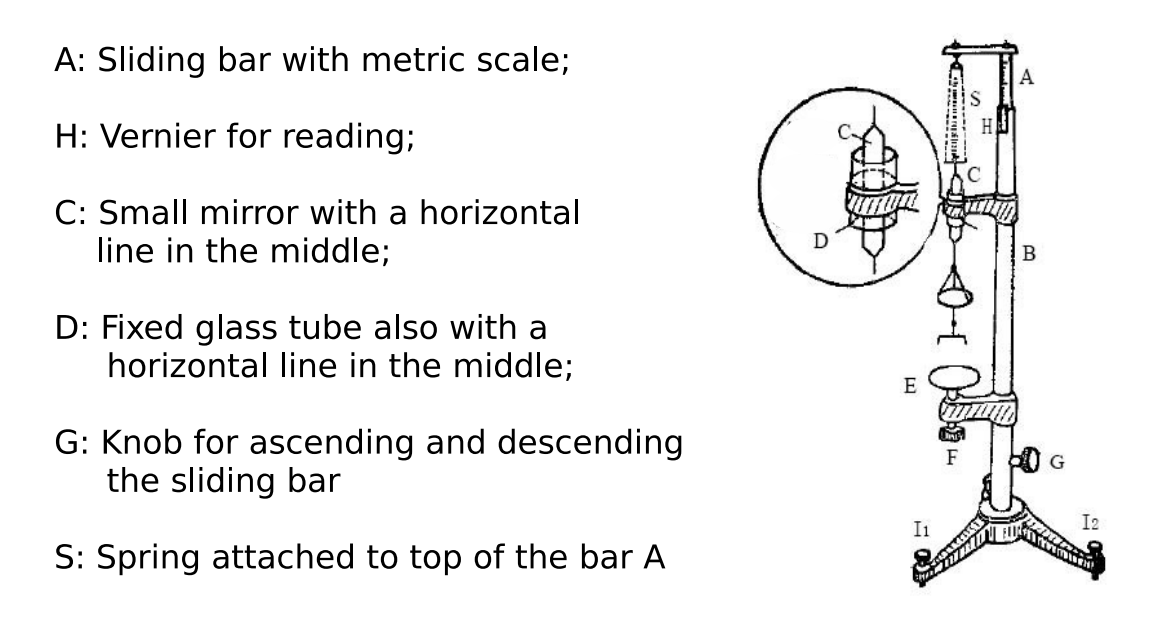
\includegraphics[scale=0.4]{jolly.png} 
        \caption{} 
        \label{jolly}
    \end{minipage} 
    \begin{minipage}[t]{0.5\linewidth}  
        \centering
        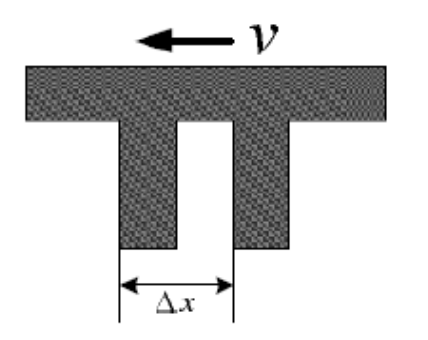
\includegraphics[scale=0.8]{U-shape.png} 
        \caption{}
        \label{ushape}
    \end{minipage} 
\end{figure}
 \newpage
 The Jolly balance measures the spring constant by reading the different scales L of the stretched spring with uncertainty of 0.02mm. \par
 The air track is used to decrease friction when the object is moving. The I shape shutter and the T mode of the electronic timer is used for timing 10 times of oscillation, with uncertainty 0.0001s. The caliper measures the outer and inner distance of the U shape shutter (figure \ref{ushape}), $x_{out}$ and $x_{in}$ with uncertainty of 0.02mm, and calculate the $\Delta x$ of travel. The U shape shutter and the S2 mode of the electronic timer measures the time $\Delta t$ it needs for the object to travel the distance $\Delta x$ with uncertainty of 0.00001s. The scale on the air track measures the amplitude A with an uncertainty of 0.1cm. The electronic balance weighs the masses, the springs, the object and U and I shape shutters with an uncertainty of 0.01g.
And a collection of those uncertainties are shown in Table \ref{apparatus}.

%----------------------------------------------------------------------------------------
\begin{table}[h]
    \centering
    \begin{tabular}{ccc}
        \toprule
    \textbf{Apparatus}   &         & \textbf{Precision} \\\hline
    \midrule    
    Jolly Balance                    &          & 0.02{[}mm{]}       \\
    Caliper                              &      & 0.02{[}mm{]}       \\
    Electronic balance                   &      & 0.01{[}g{]}        \\
    \multirow{2}{*}{Photoelectric measuring system} & Mode $T$   & 0.0001{[}s{]}       \\
                                   & Mode $S_2$ & 0.00001{[}s{]}     \\
    Air track                         &         & 0.1{[}cm{]}       \\\bottomrule
    \end{tabular}
    \caption{Apparatus Uncertainty}
    \label{apparatus}
    \end{table}


%---------------------------------------------------------------------
%SECTION 4
%---------------------------------------------------------------------
\section{Measurement Procedure}
\subsection{Spring Constant}
\begin{enumerate}[1.]
    \item  Adjust the Jolly balance to be vertical. The method is to add some preload first. Make sure the mirror on the jolly balance (figure \ref{jolly}) can move freely ,the spring is parallel to the Jolly balance and the mirror doesn't touch the edge of the tube.
    \item Add adjust knob and make 3 lines coincide. Adjust the tube to set the initial position $L_0$ within 5.0 ~ 10.0 cm.
    \item Record the reading $L_0$ on the scale, add mass $m_1$ and record $L_1$.
    \item Keep adding masses and measure six positions.
    \item Estimate the spring constant $k_1$
    \item Replace spring 1 with spring 2, repeat the measurements.
\end{enumerate}
\subsection{Relation Between the Oscillation Period T and the Mass of the Oscillator M}
\begin{enumerate}[1.]
    \item Adjust the air track so that it is horizontal.
        \begin{itemize}
            \item [\romannumeral 1] Turn on the air pump and all the holes work well.
            \item [\romannumeral 2] Place the object on the track without initial velocity. Adjust the track until the object moves slowly back and forth in both directions.
        \end{itemize}
    \item Horizontal air track
        \begin{itemize}
            \item [\romannumeral 1]  Attach springs to the sides of the cart, and set up the I-shape shutter. Make sure
            that the photoelectric gate is at the equilibrium position.
            \item[\romannumeral 2]  Add mass in an unchanged order for 6 times and make small oscillations with amplitude
            about 5cm. Set the timer to T mode to test the interval for the object to travel 10 periods of
            oscillations.
        \end{itemize}
    \item Inclined air track\par
    Place plastic plates under one side of the track to create inclined platform. First place 3 plates and then place 6 plates. Repeat steps in Horizontal air track.
        \item Plot graphs to find the relationship between $M$ and $T^2$.
\end{enumerate}
\newpage
\subsection{Relation Between the Oscillation Period T and the Amplitude A}
\begin{enumerate}[1.]
    \item  Keep the mass of the object unchanged and change the amplitude of the oscillations. The
    recommended amplitude is 5.0/10.0/15.0/20.0/25.0/30.0 cm.
    \item Record the period and apply linear fit to find whether T and A are related.
\end{enumerate}
\subsection{ Relation Between the Maximum Speed and the Amplitude}
\begin{enumerate}[1.]
    \item  Measure the outer distance $x_{out}$ and the inner distance $x_{in}$ of the U-shape shutter by
    a caliper. Calculate the distance $\Delta x=(x_{in}+x_{out})/2$.
    \item Change the shutter from I- to U-shape. Set the timer into the ”S2” mode. Let the cart
    oscillate. Record the second readings of the time interval $\Delta t$ only if the two subsequent
    readings show the same digits to the left of the decimal point.
    \item Change the amplitude 5 times recommended to be 5.0/ 10.0/ 15.0/ ... /30.0 cm.
    \item  Measure the maximum speed $v_{max}$ for different values of the amplitude A and obtain the spring constant. Compare this result to that of the first part.
\end{enumerate}
\subsection{Mass measurement}
\begin{enumerate}[1.]
    \item Adjust the electronic balance.
    \item Add weights according to a fixed order. Weigh the cart with the I-shape shutter and
    with the U-shape shutter. Measure the mass of spring 1 and spring 2.
    \item Record the data only after the circular symbol on the scales display disappears.
\end{enumerate}
%----------------------------------------------------------------------------------------
%	SECTION 6
%----------------------------------------------------------------------------------------

\section{Results}
\subsection{Measurement of the spring constant}
\qquad The procedure of measuring the spring constant is mentioned in part 3.1 and the measuring of masses is mentioned in part 3.5. Transfer the measured data to SI units and we can get two tables for L (Table \ref{measurespringconstant}) and mass (Table \ref{massofthemasses}), and we further calculate $\Delta_L$ with the initial $L_0$, shown in Table \ref{deltal} and the value of mg, taking $g=9.794m/s^2$, shown in Table \ref{mg}. Recall that $k=mg/x$, so we do the linear fit of points ($\Delta L,m$), and we get our k. The figures are shown in Figure \ref{constantfigure}\par
$\ $Read from the graph we can directly get the value of k (slope) and the uncertainty of k (CI Half-Width).
\begin{equation*}
    k_1= 1.66\pm 0.03[N/m]\ \ \ k_2=1.66\pm 0.03[N/m]
\end{equation*}

\begin{center}
    \begin{figure}[H]
        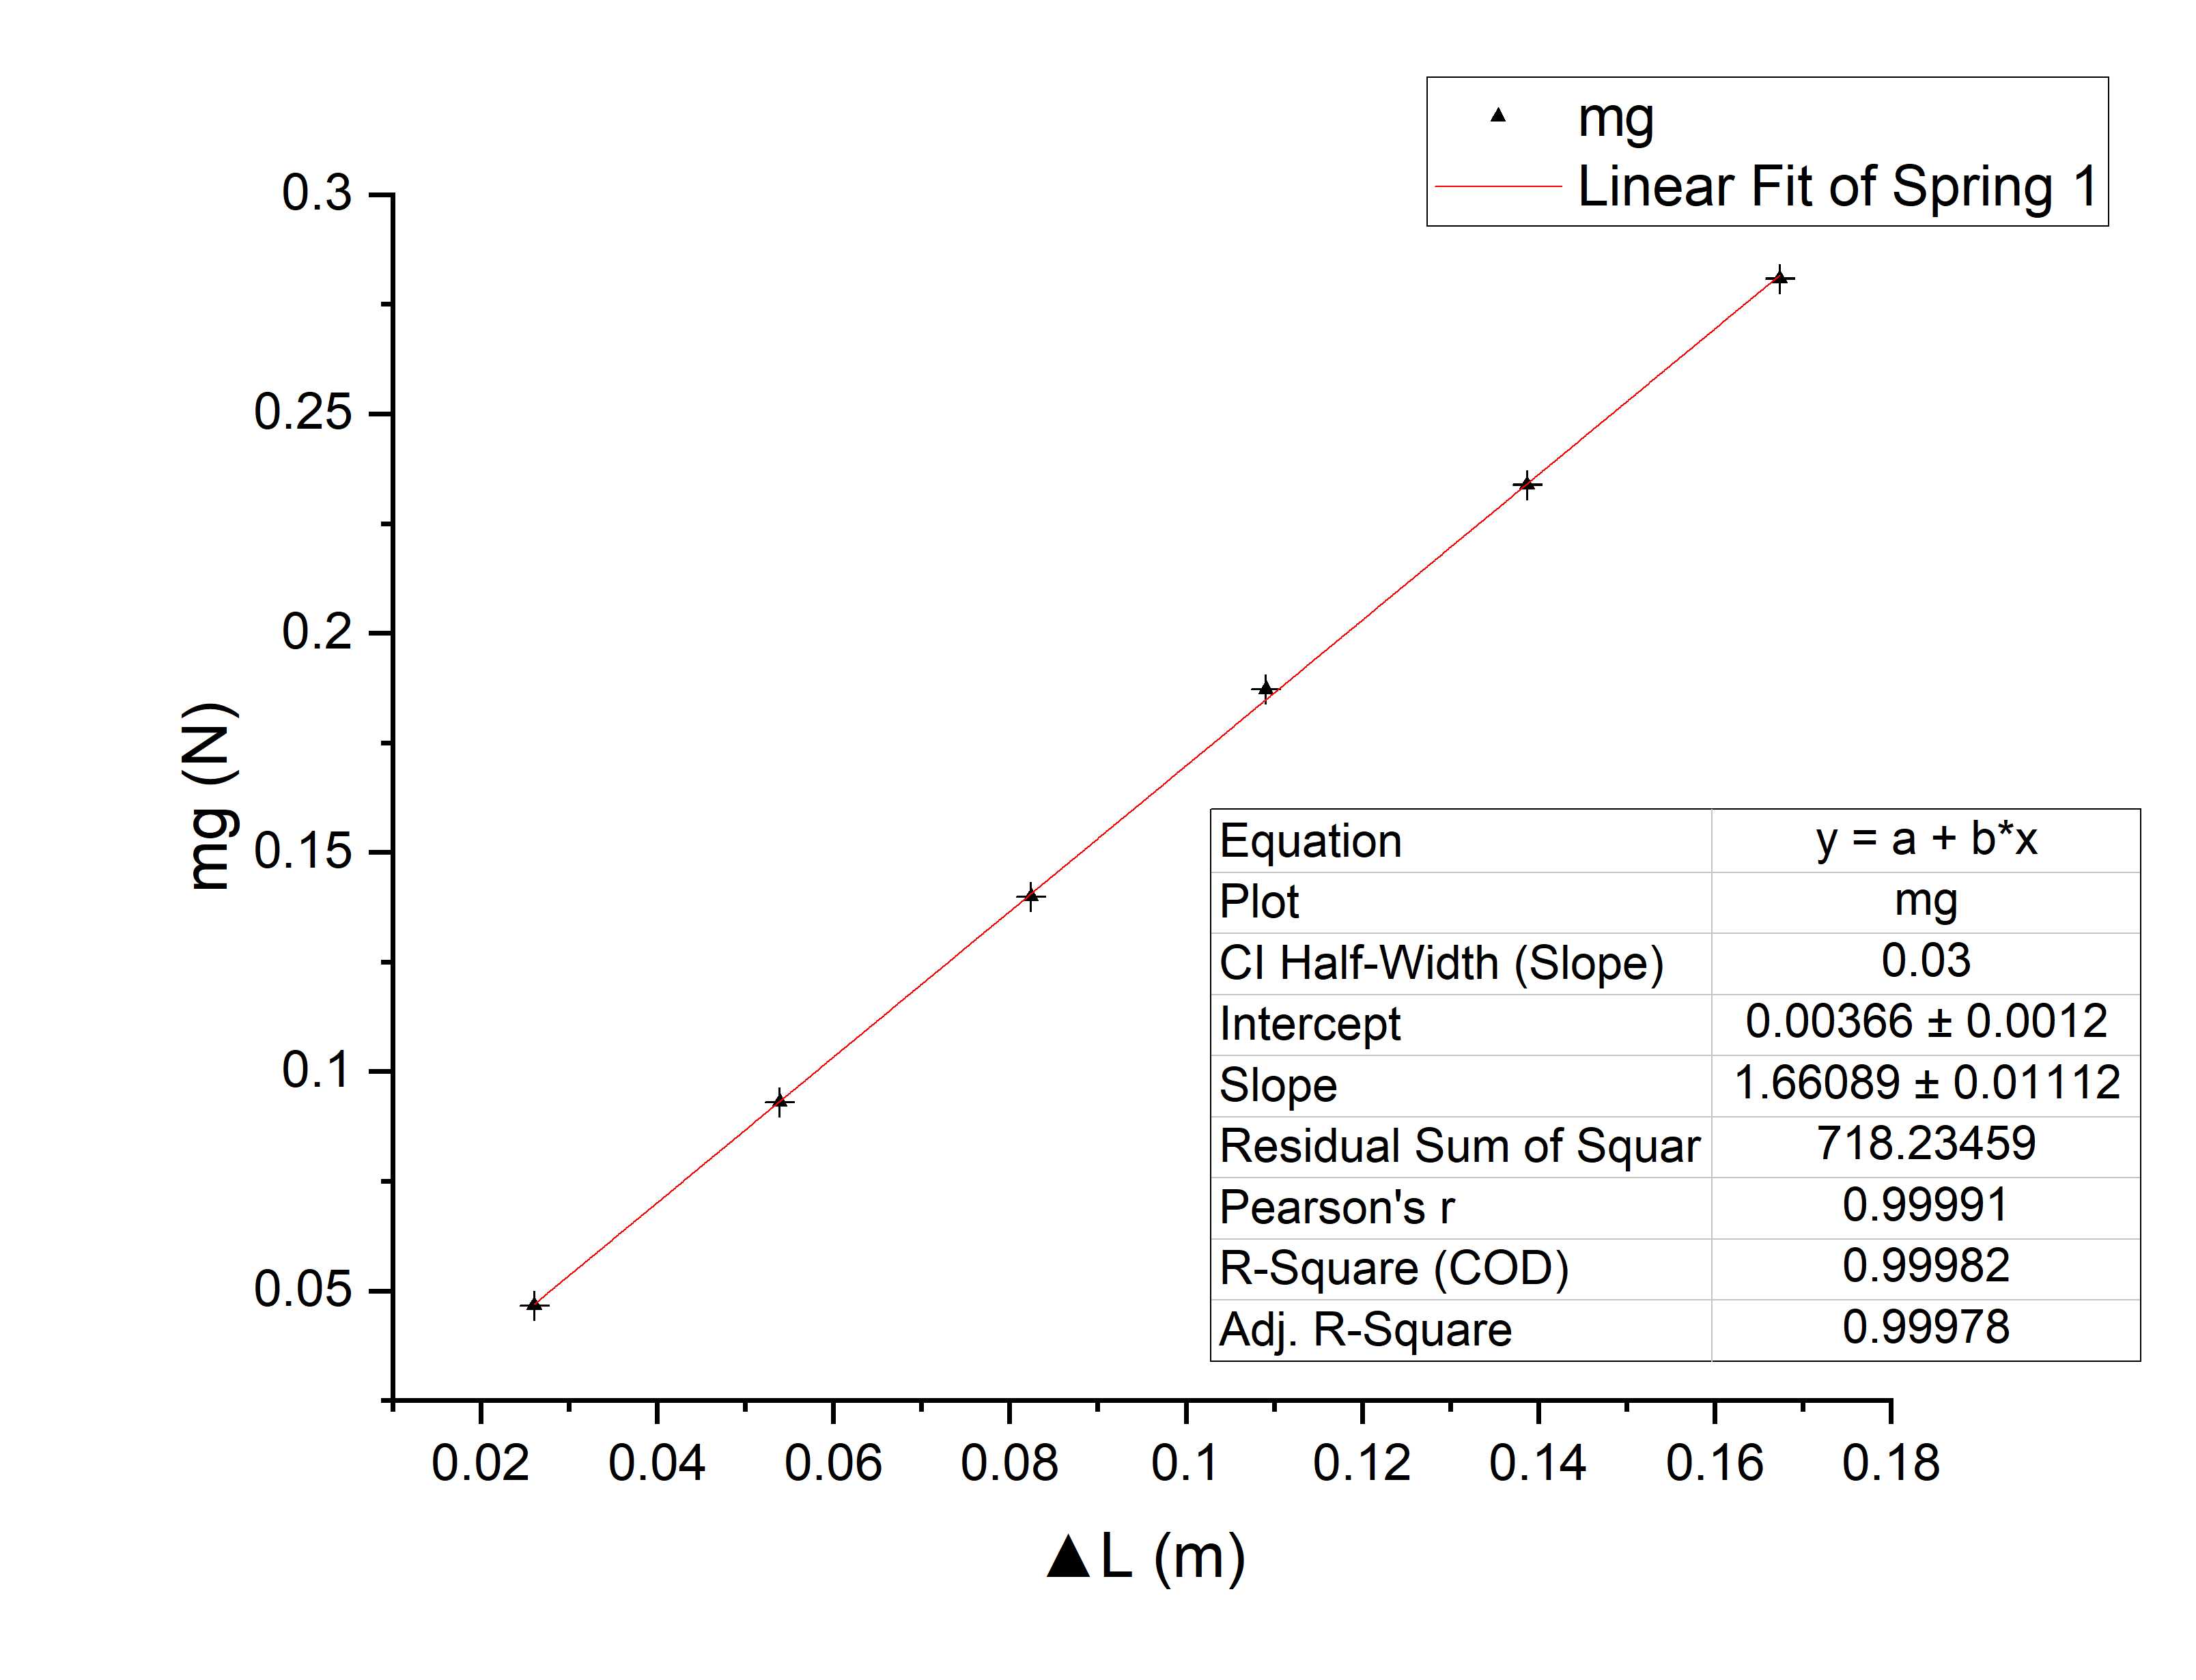
\includegraphics[scale=0.35]{spring1-delta.png}
    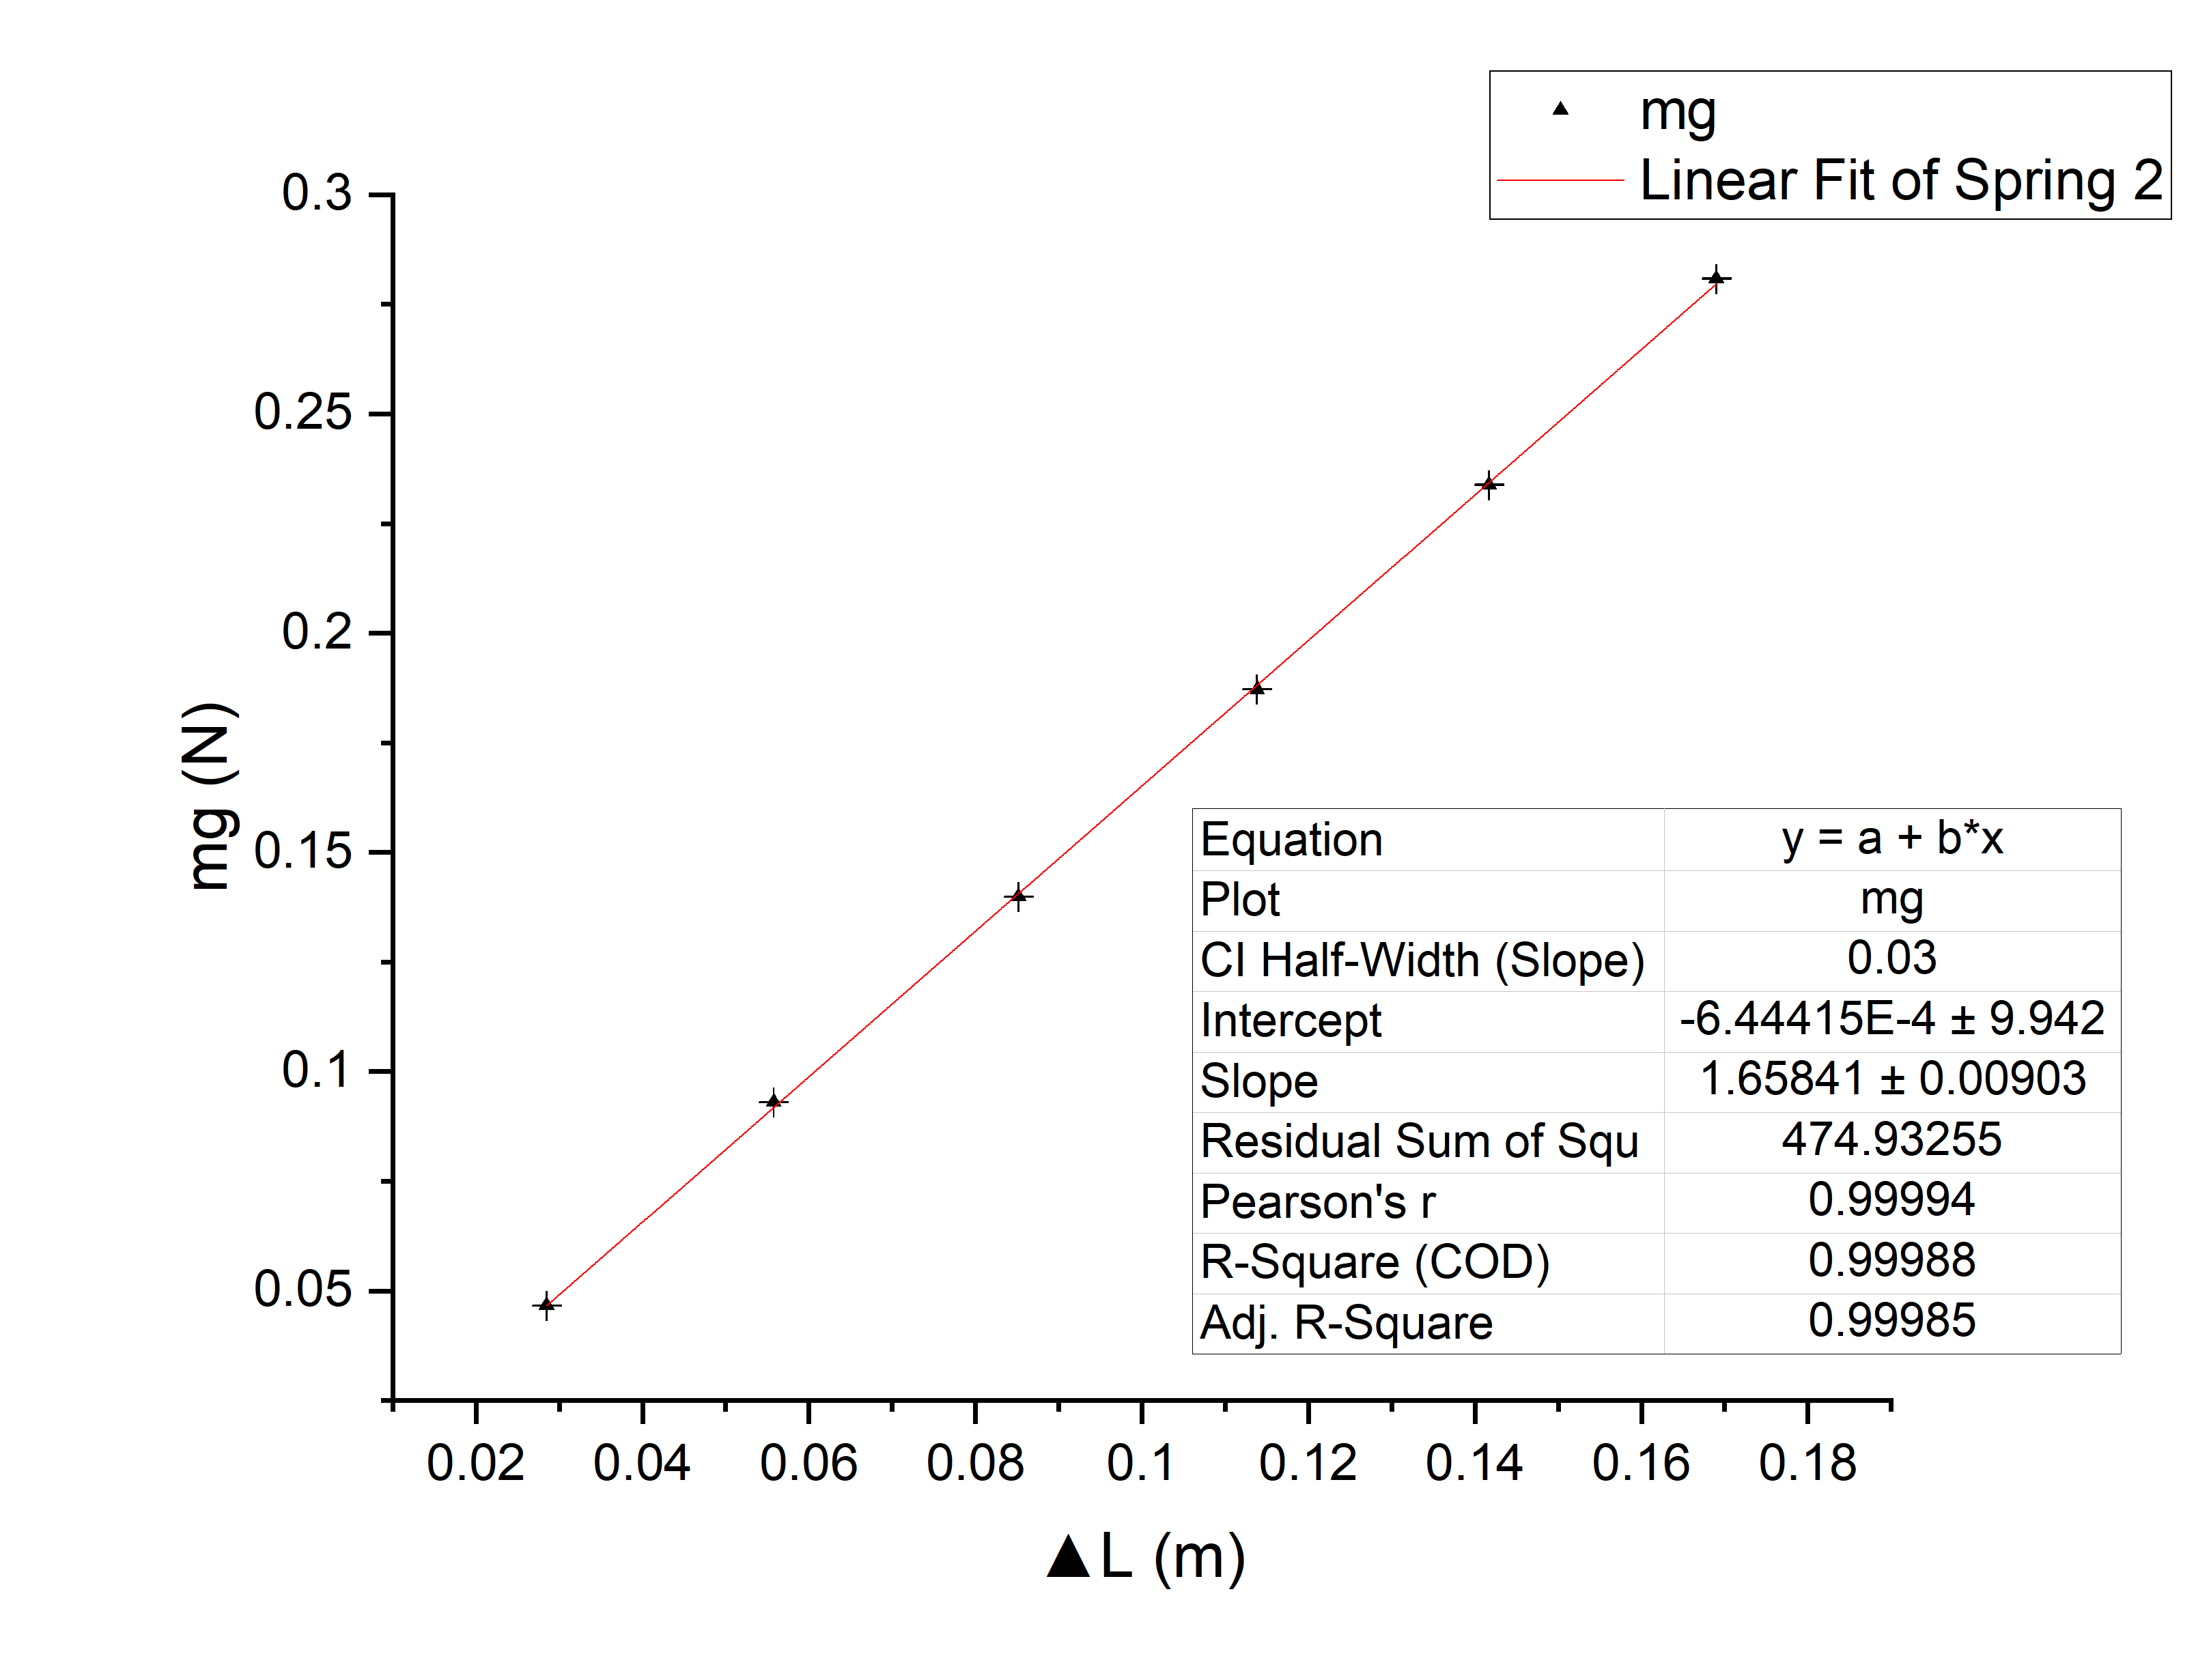
\includegraphics[scale=0.35]{spring2-delta.png}
    \caption{The linear fit figures of spring 1, 2}
    \label{constantfigure}
    \end{figure}
\end{center}
\subsection{Analyzing the Relation Between T and Mass of the Oscillator M}
\qquad The procedure of measuring T and M are shown respectively in 3.2 and 3.5. Here we use the mass of the sum of equivalent mass of I-shape and the masses, shown in Table \ref{equivalent2}. And for T, we first get T from $T_{10}$ (see Table \ref{valuettm}) and then we calculate the value of $T^2$, shown in Table \ref{valueT2}, note that the uncertainty varies with T, so that the uncertainty of it is listed in another table \ref{uncertainty of Tsquare}.\par
$\ $Therefore,we can study the relation between T and M(Table \ref{equivalent2}) by linear fit $T^2$ with M, as shown in figure \ref{tmfigure}.\\
Directly from the figure, we can read the slope, which means the value and uncertainty of $T^2/m$, the three values are respectively:$$11.795\pm 0.015,\ \ 11.826\pm 0.030,\ \ 11.82\pm 0.04\ \ [s^2/kg]$$
\begin{center}
    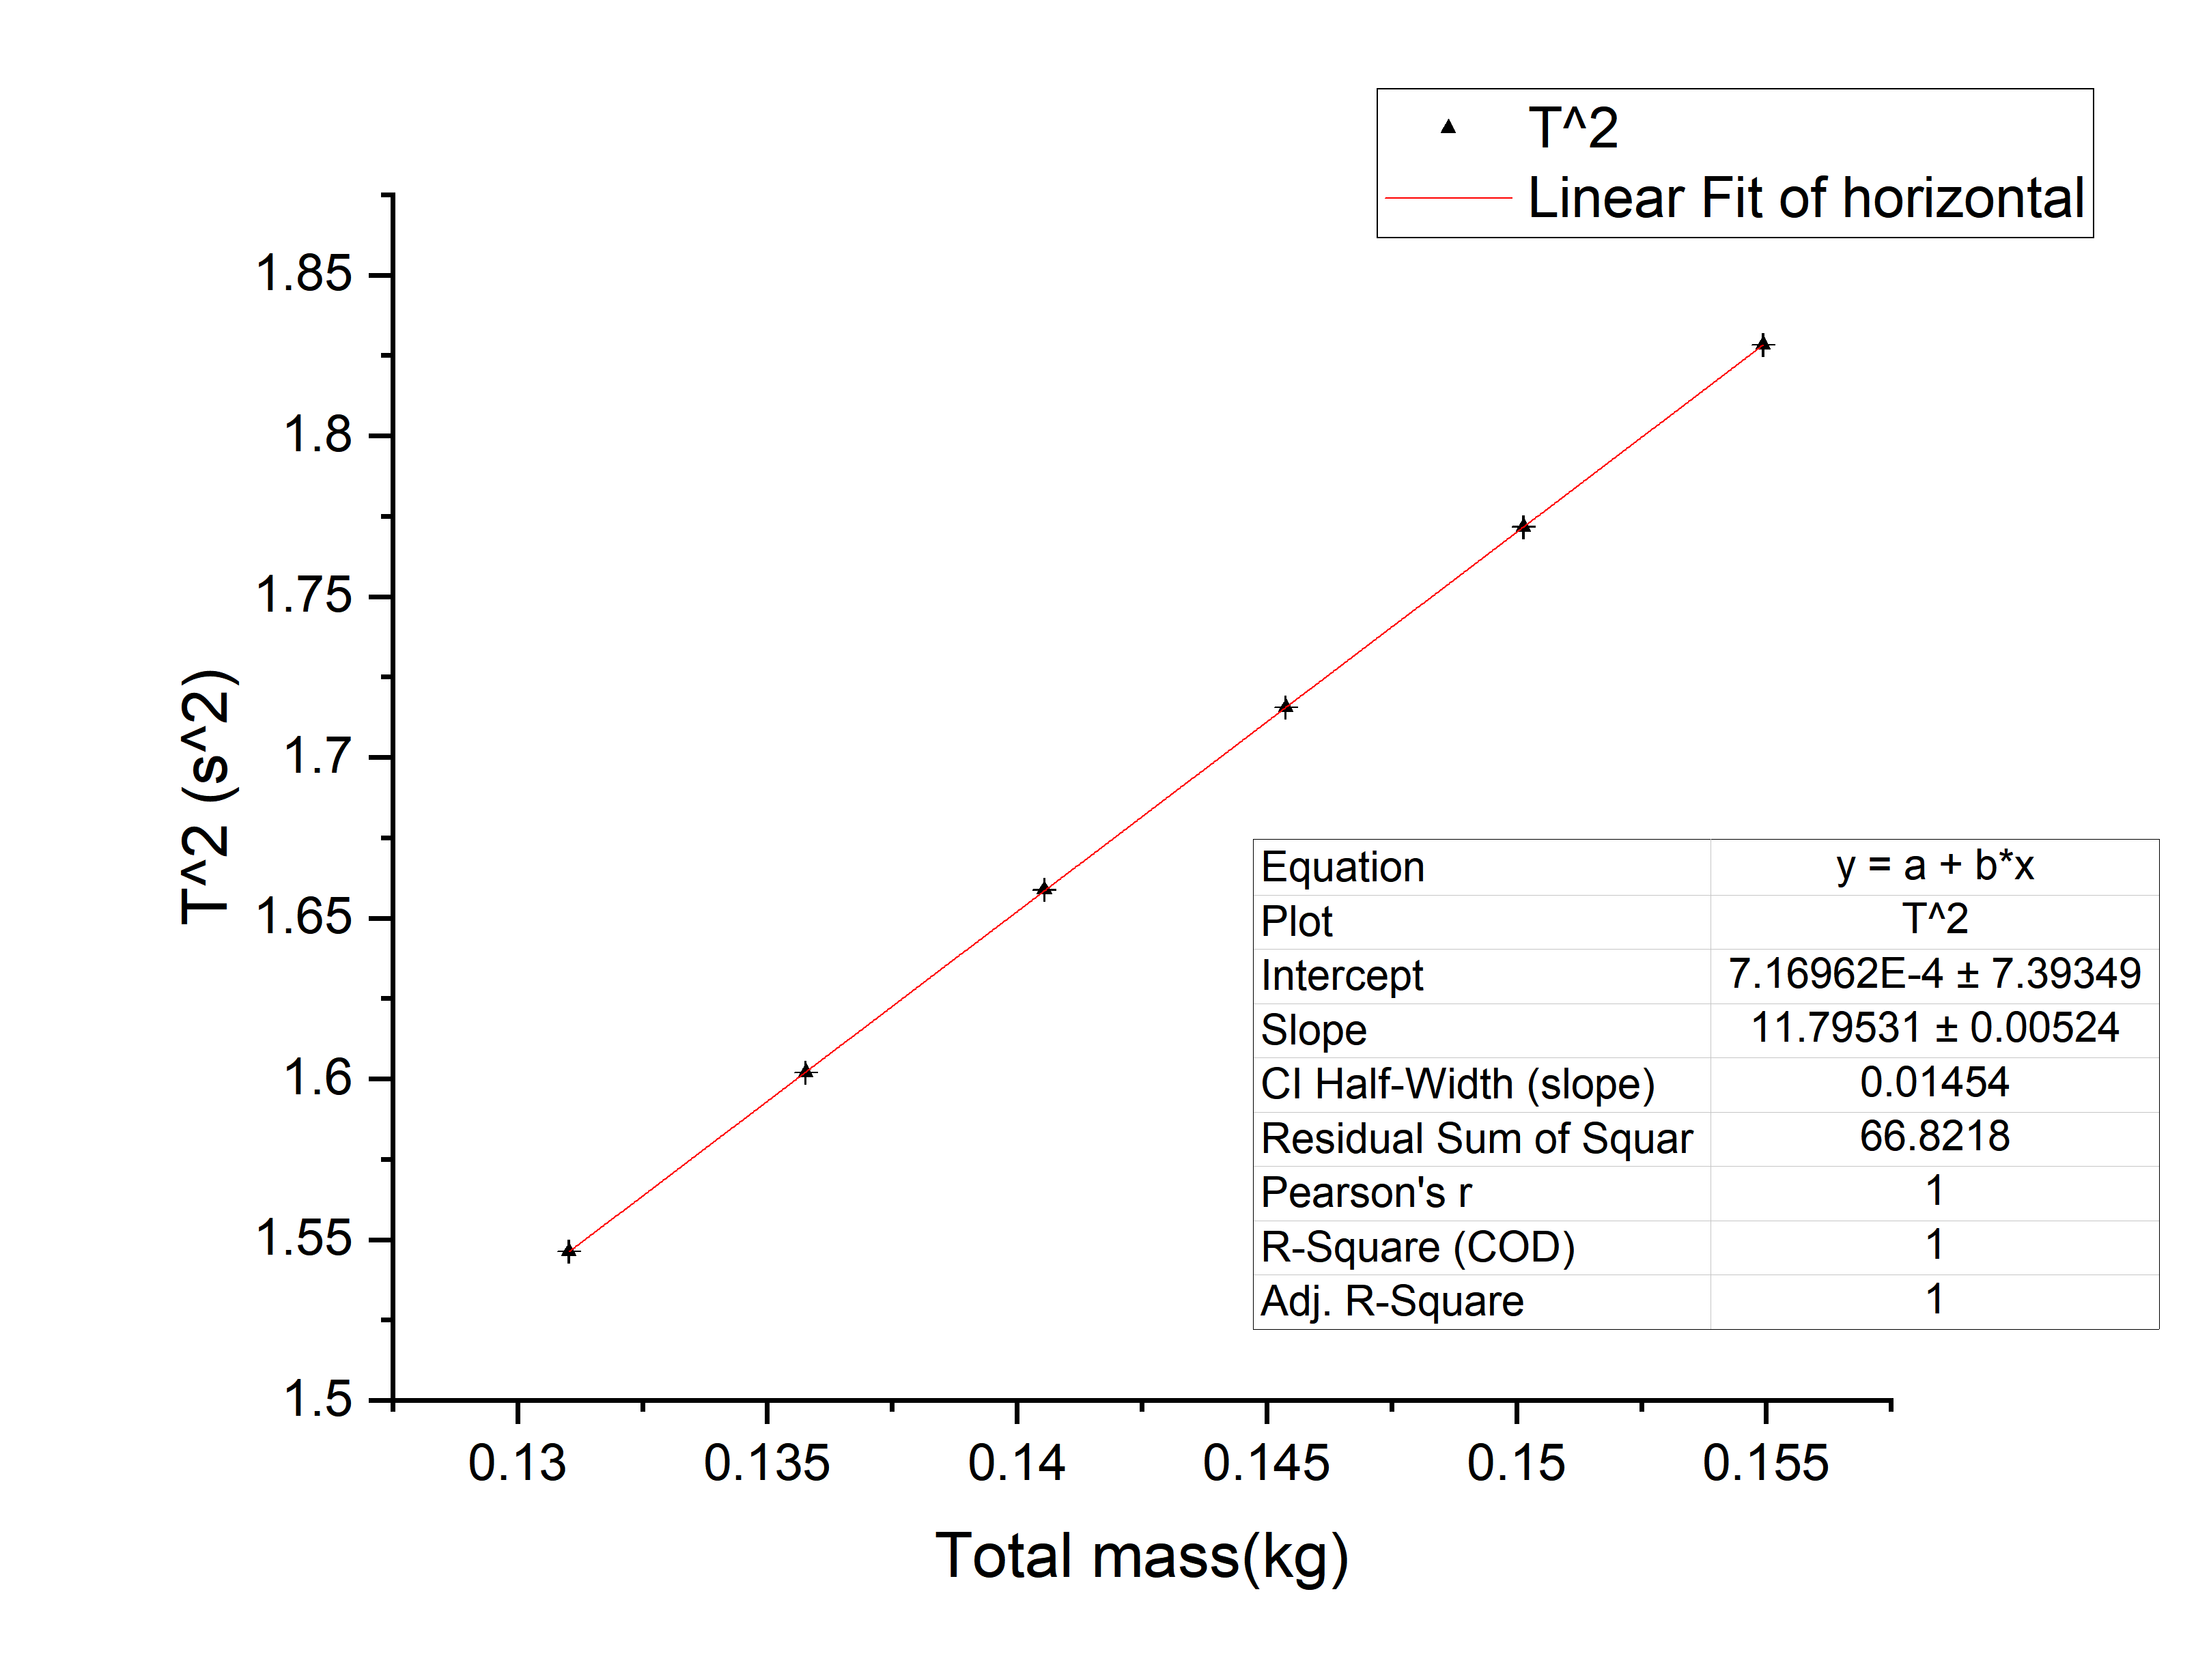
\includegraphics[scale=0.4]{horizontal.png}

    \begin{figure}[H]
            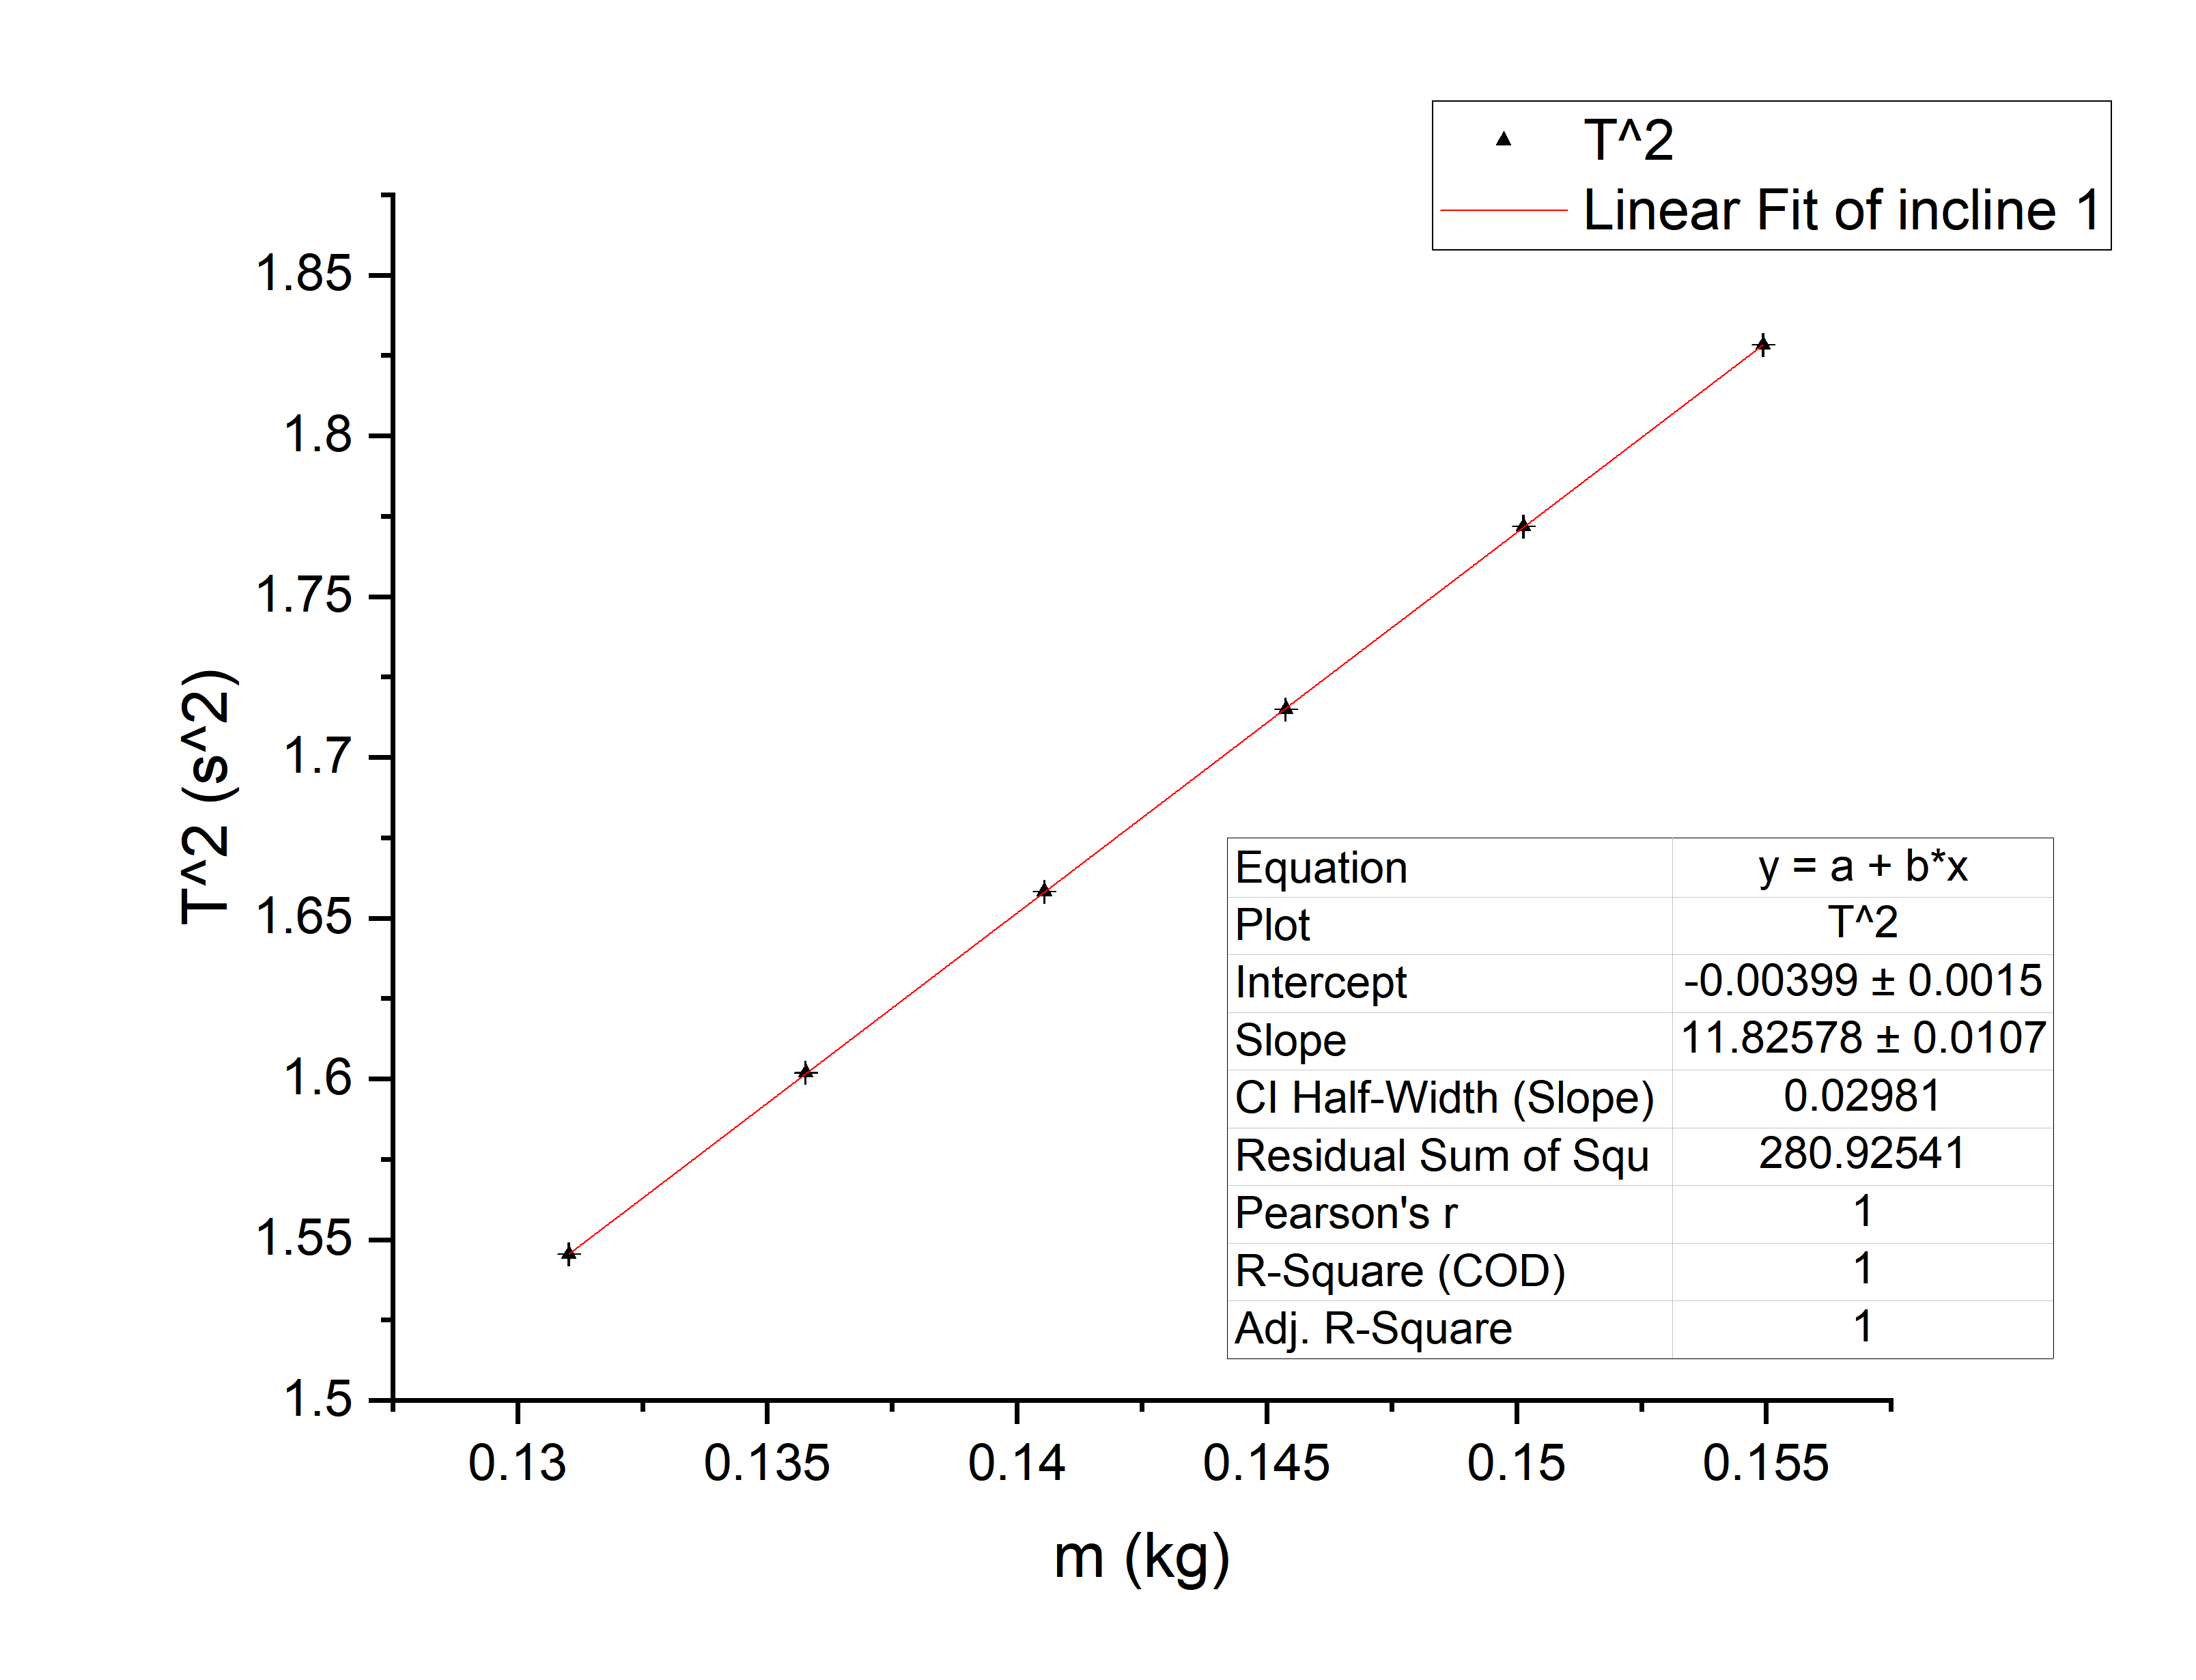
\includegraphics[scale=0.35]{incline1.png}
    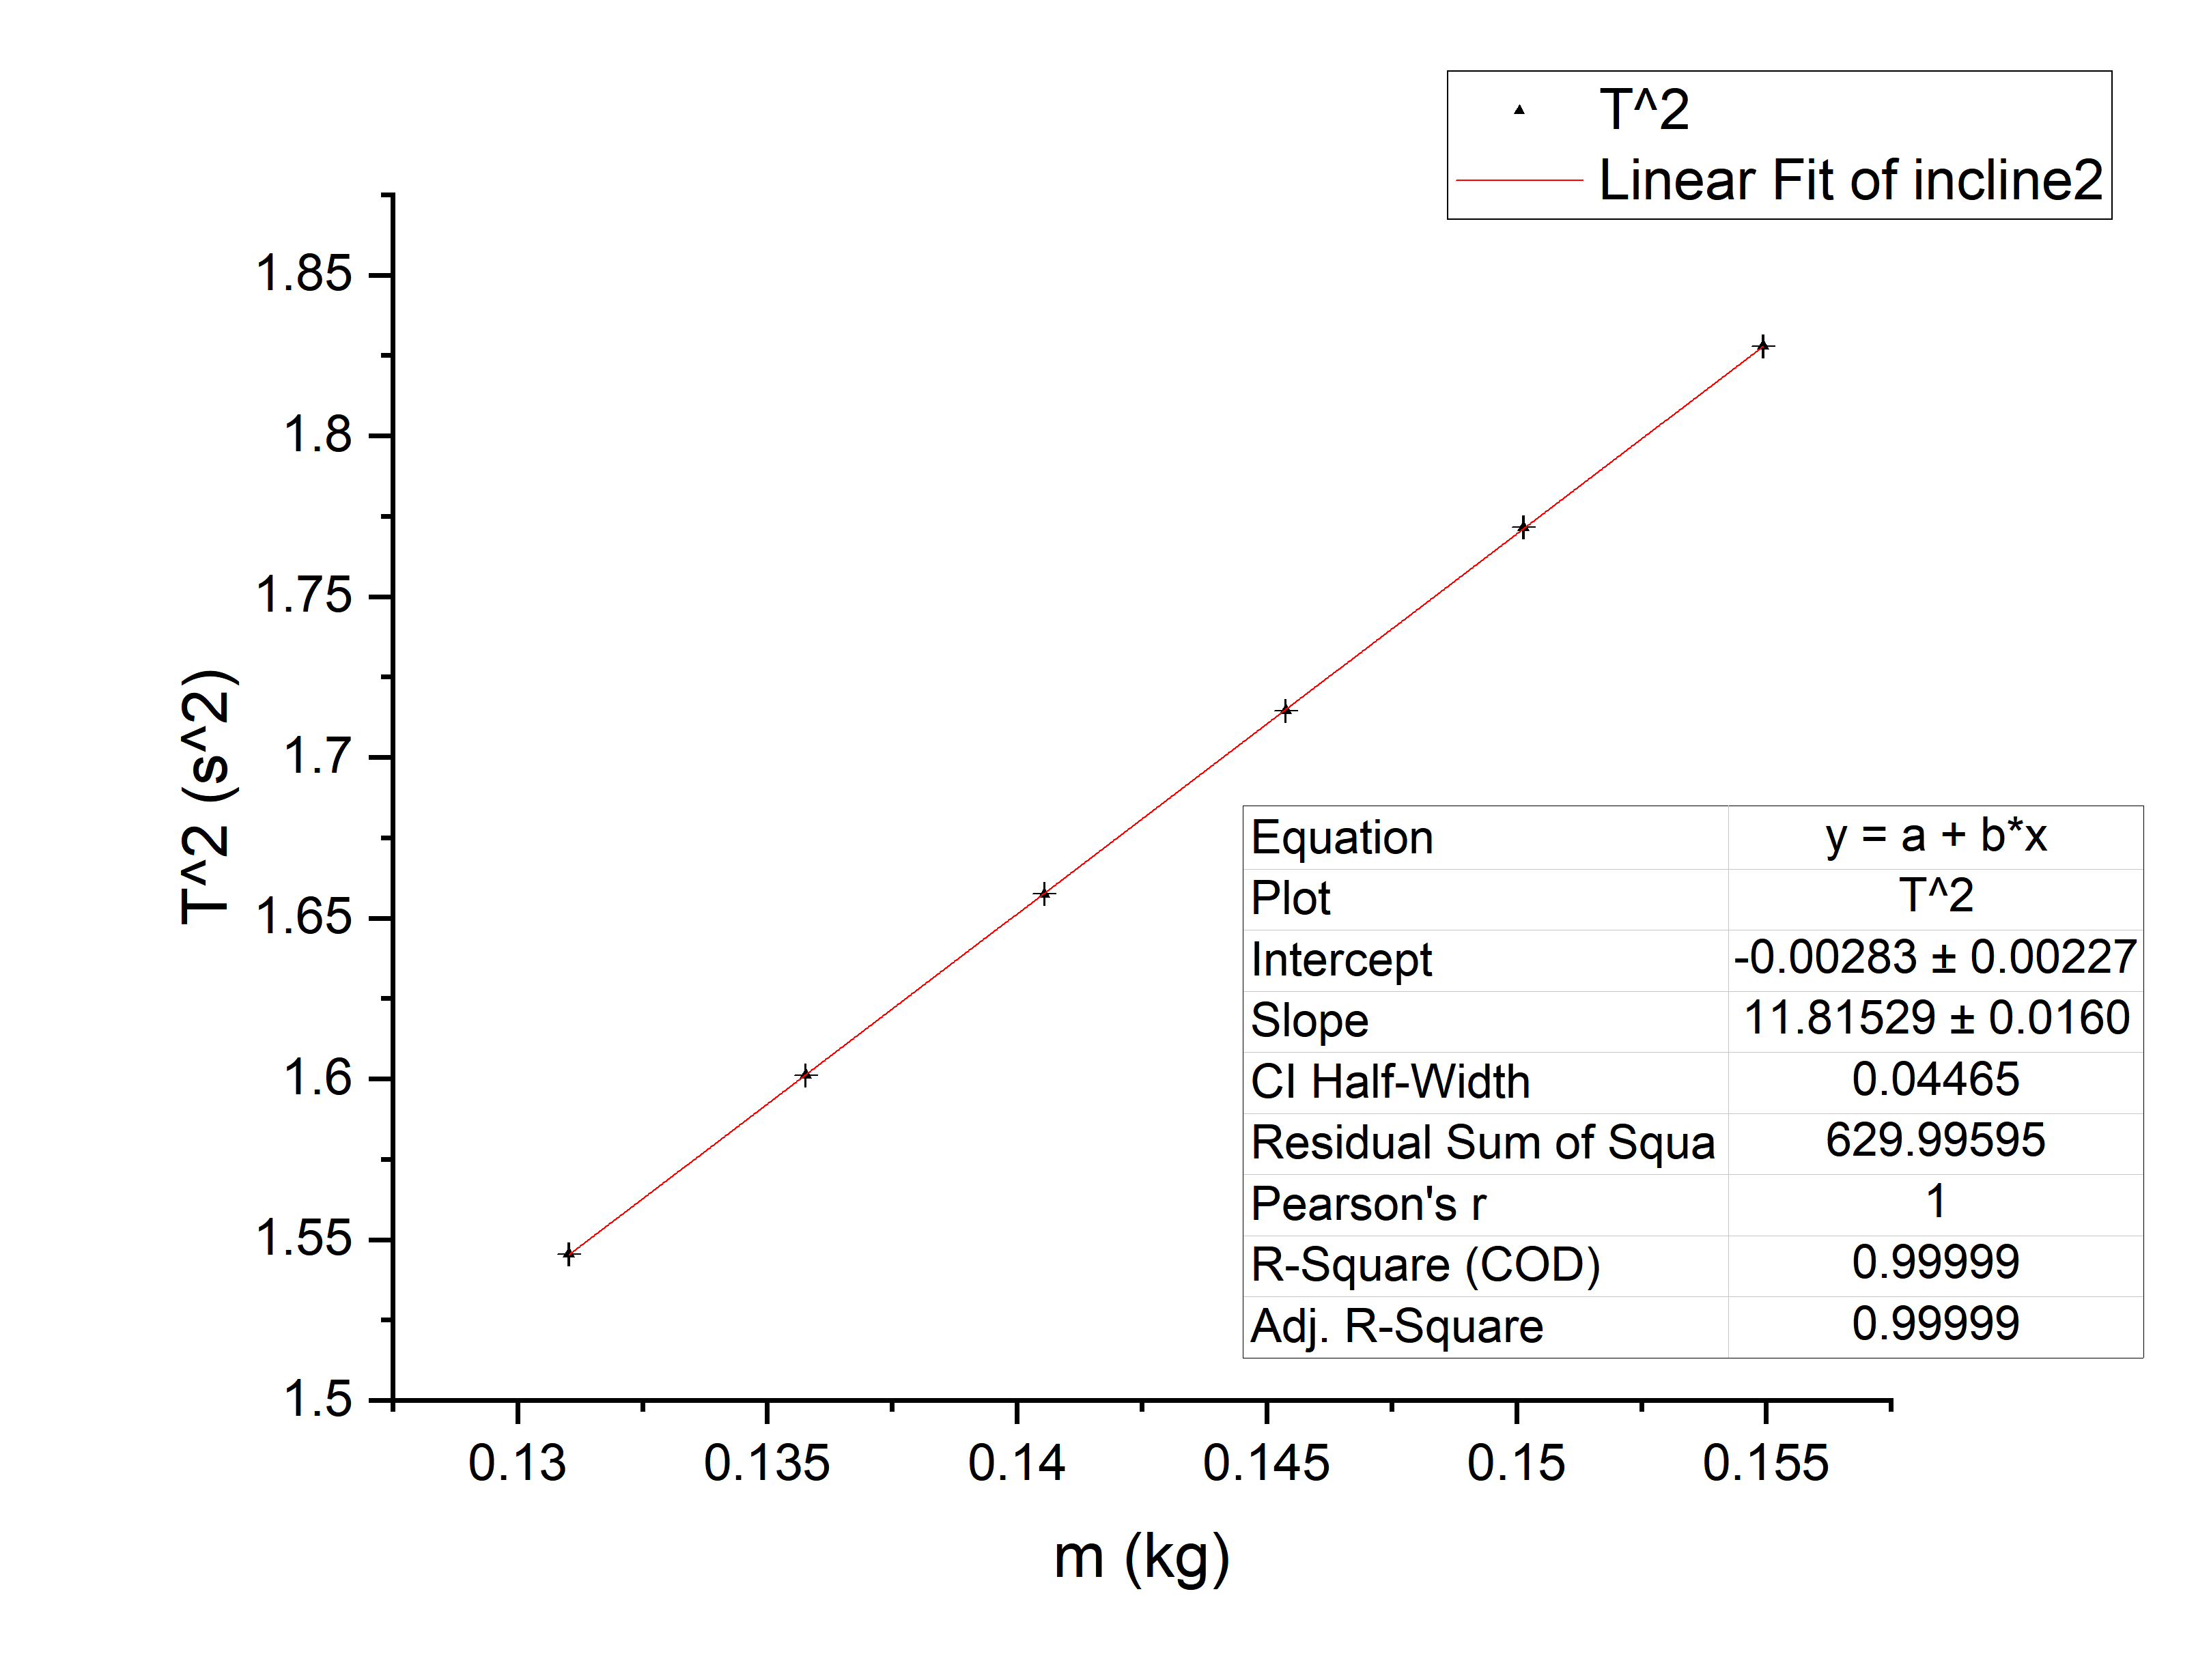
\includegraphics[scale=0.35]{incline2.png}
    \caption{Linear fit of $T^2/m$ for horizontal, incline 1, incline 2 air track.}
    \label{tmfigure}
    \end{figure}
\end{center}
\qquad From the graphs we can see that the three fitted k don't have obvious differences. Recall that $\frac{T^2}{M}=4\pi^2\cdot \frac{1}{k_1+k_2}$, so we can get the theoretical value of $\frac{T^2}{M}$ to be:$$\frac{T^2}{M}=4\pi^2\cdot \frac{1}{1.66+1.66}=11.9\pm 0.15[s^2/kg]$$
So that the relative difference of the three fitted value is respectivly: $0.81\%,\ 0.55\%,\ 0.64\%$, so that the fitted values are close to the theoretical value.
\subsection{Analyzing the Relation Between Period T and Amplitude A}
\qquad The procedure of measuring T and A are mentioned in part 3.3. The table of T and A in this part are listed together in Tabel \ref{TADATA}. The graph of A and T is shown in figure \ref{figureAT}: we can see from the graph that there's no obvious relationship of A and T, and the correlation coefficient($\gamma=0.25$)
\begin{figure}[H]
    \centering
    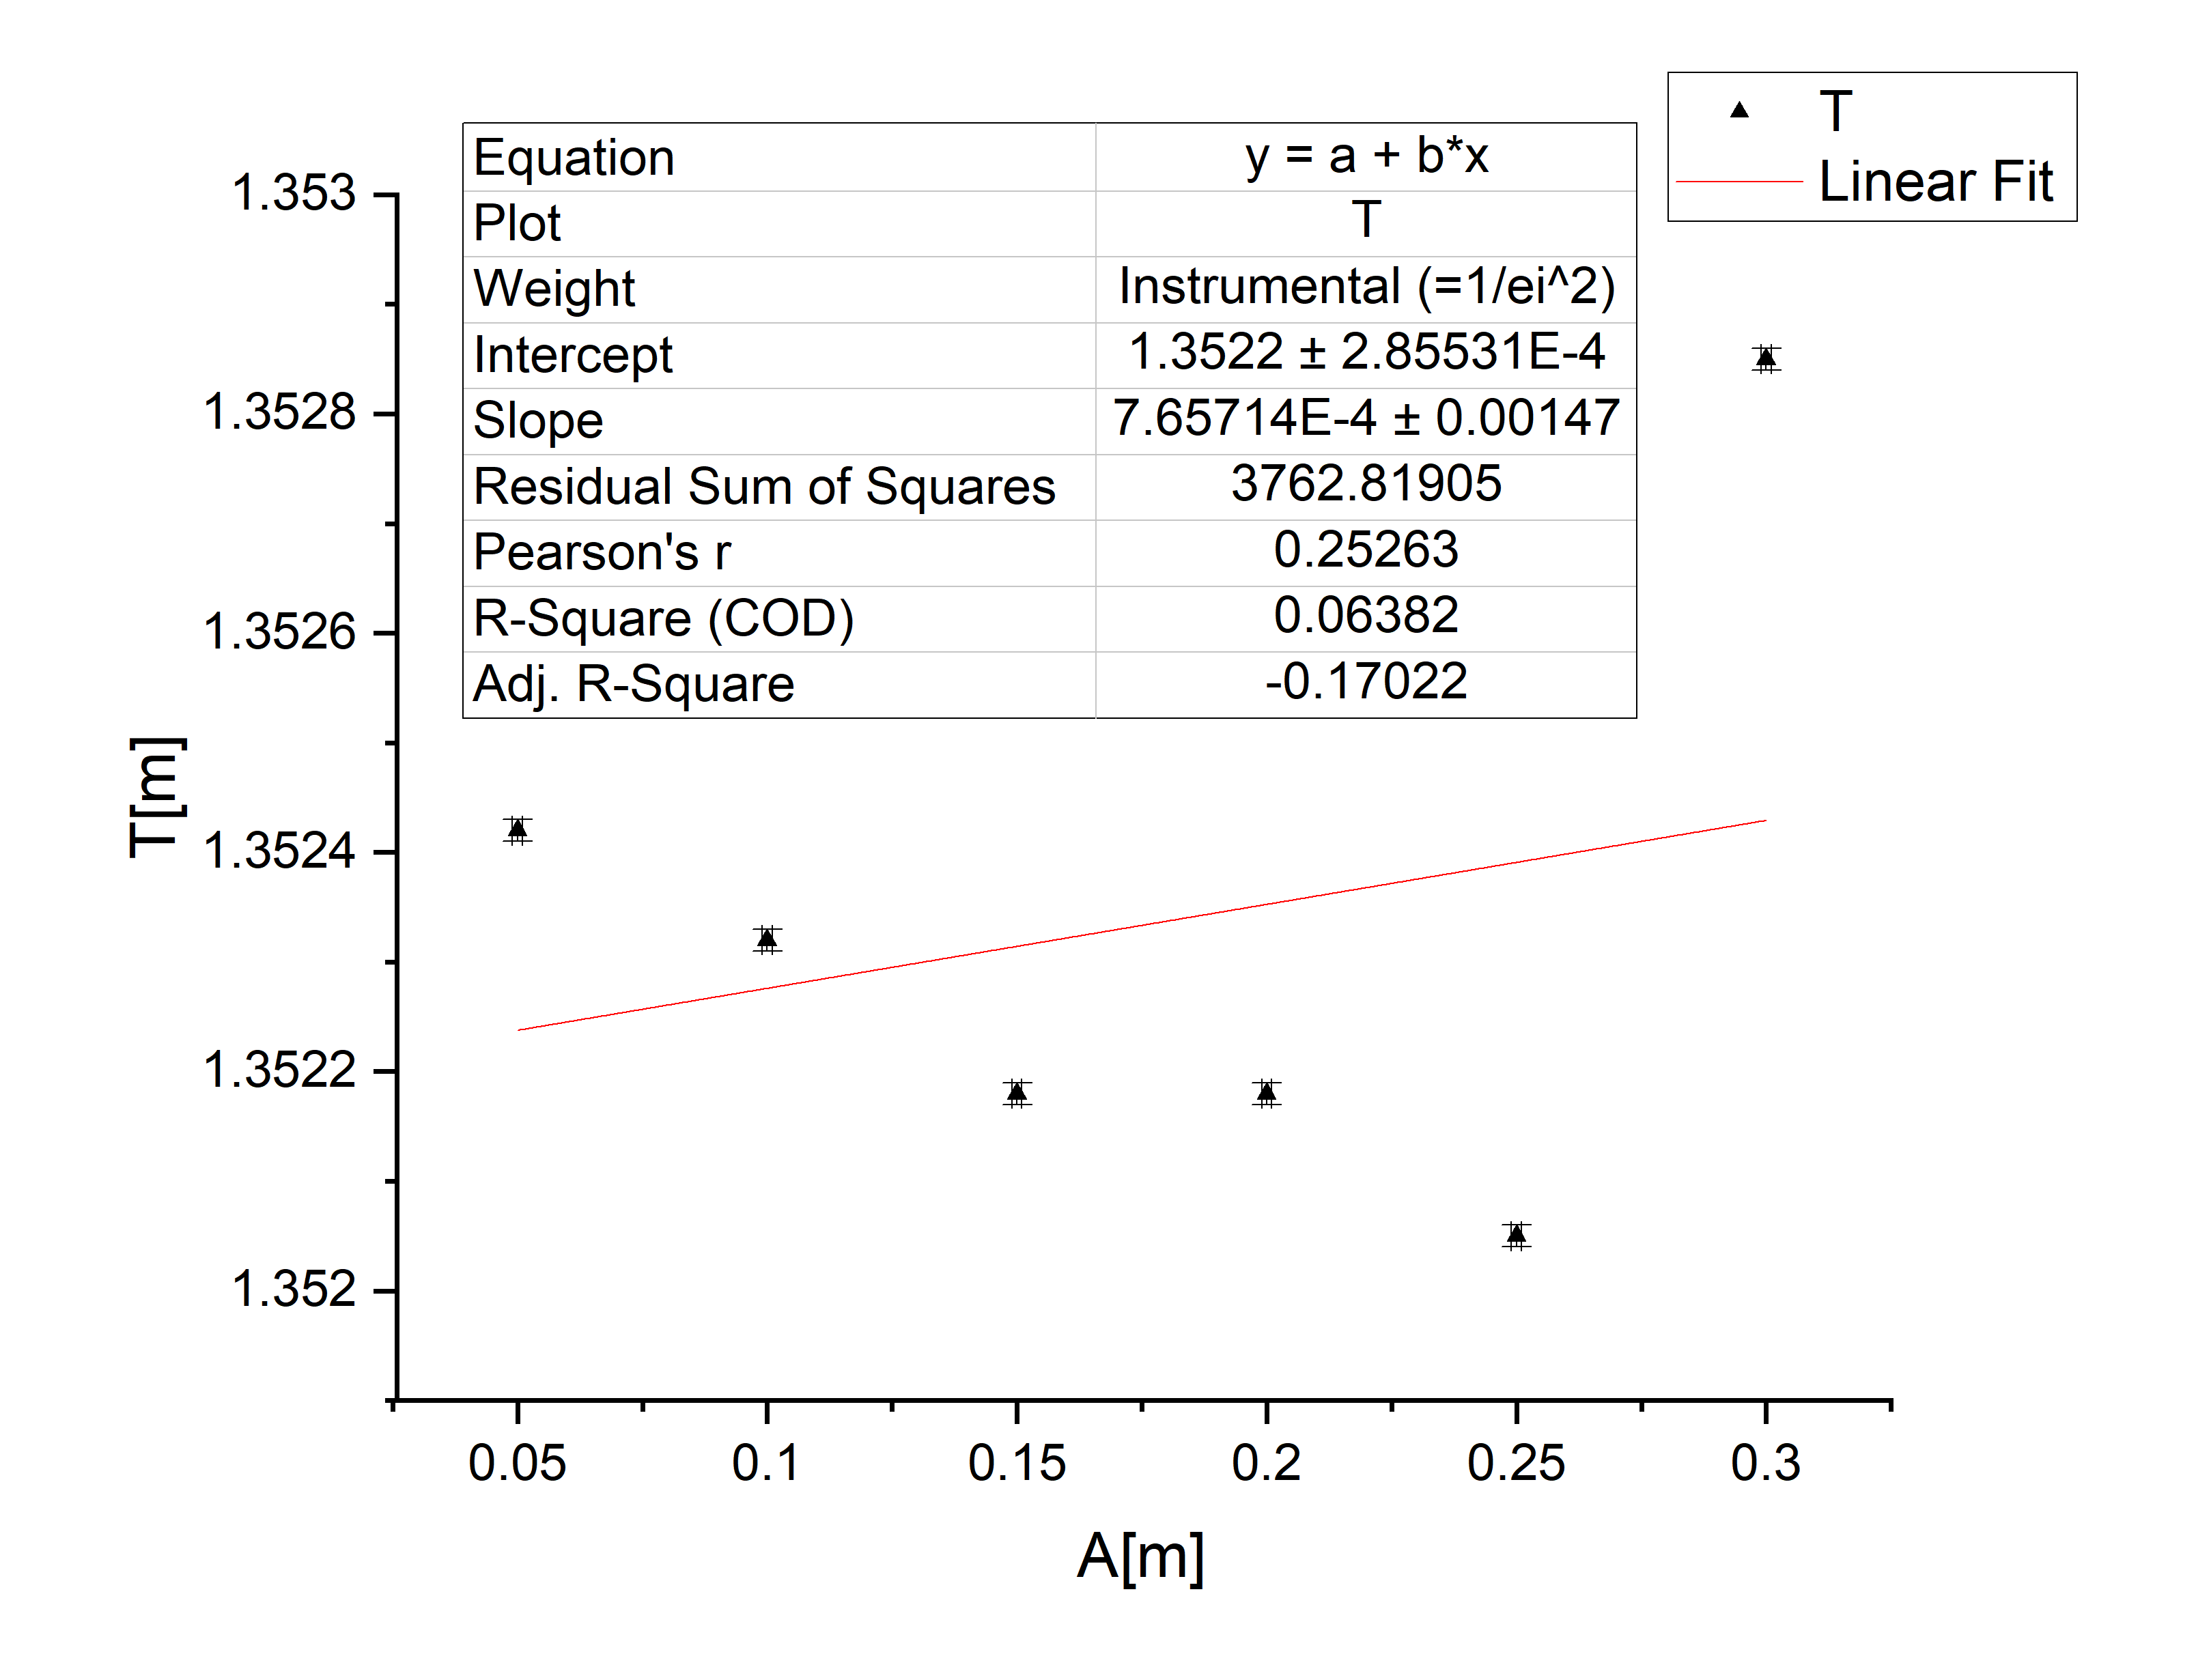
\includegraphics[scale=0.4]{TvsA.png}
    \caption{Relation between A and T}
    \label{figureAT}
\end{figure}


\subsection{Analyzing the Relation Between Maximum Speed and Amplitude}
\qquad To calculate speed, we get it from $v=\Delta x/\Delta t$, and $\Delta x=\frac{1}{2}(x_{in}+x_{out})$, and we get $\Delta x=0.01000\pm 0.00004[m]$. Hence we list the value of A, v in Table \ref{AandV}. Note that the uncertainty of v varies with the value of v, so that the uncertainty for v is listed in table \ref{uncertainty of mu v}.\par
$\ $ Since we are to plot the figure of $mv^2$ vs. $A^2$, we then calculate the value of $mv^2$ and $A^2$ and their uncertainties, which are all listed in Table \ref{valuemv2a2}. The graph is shown in Figure \ref{mva}
\begin{figure}[H]
    \centering
    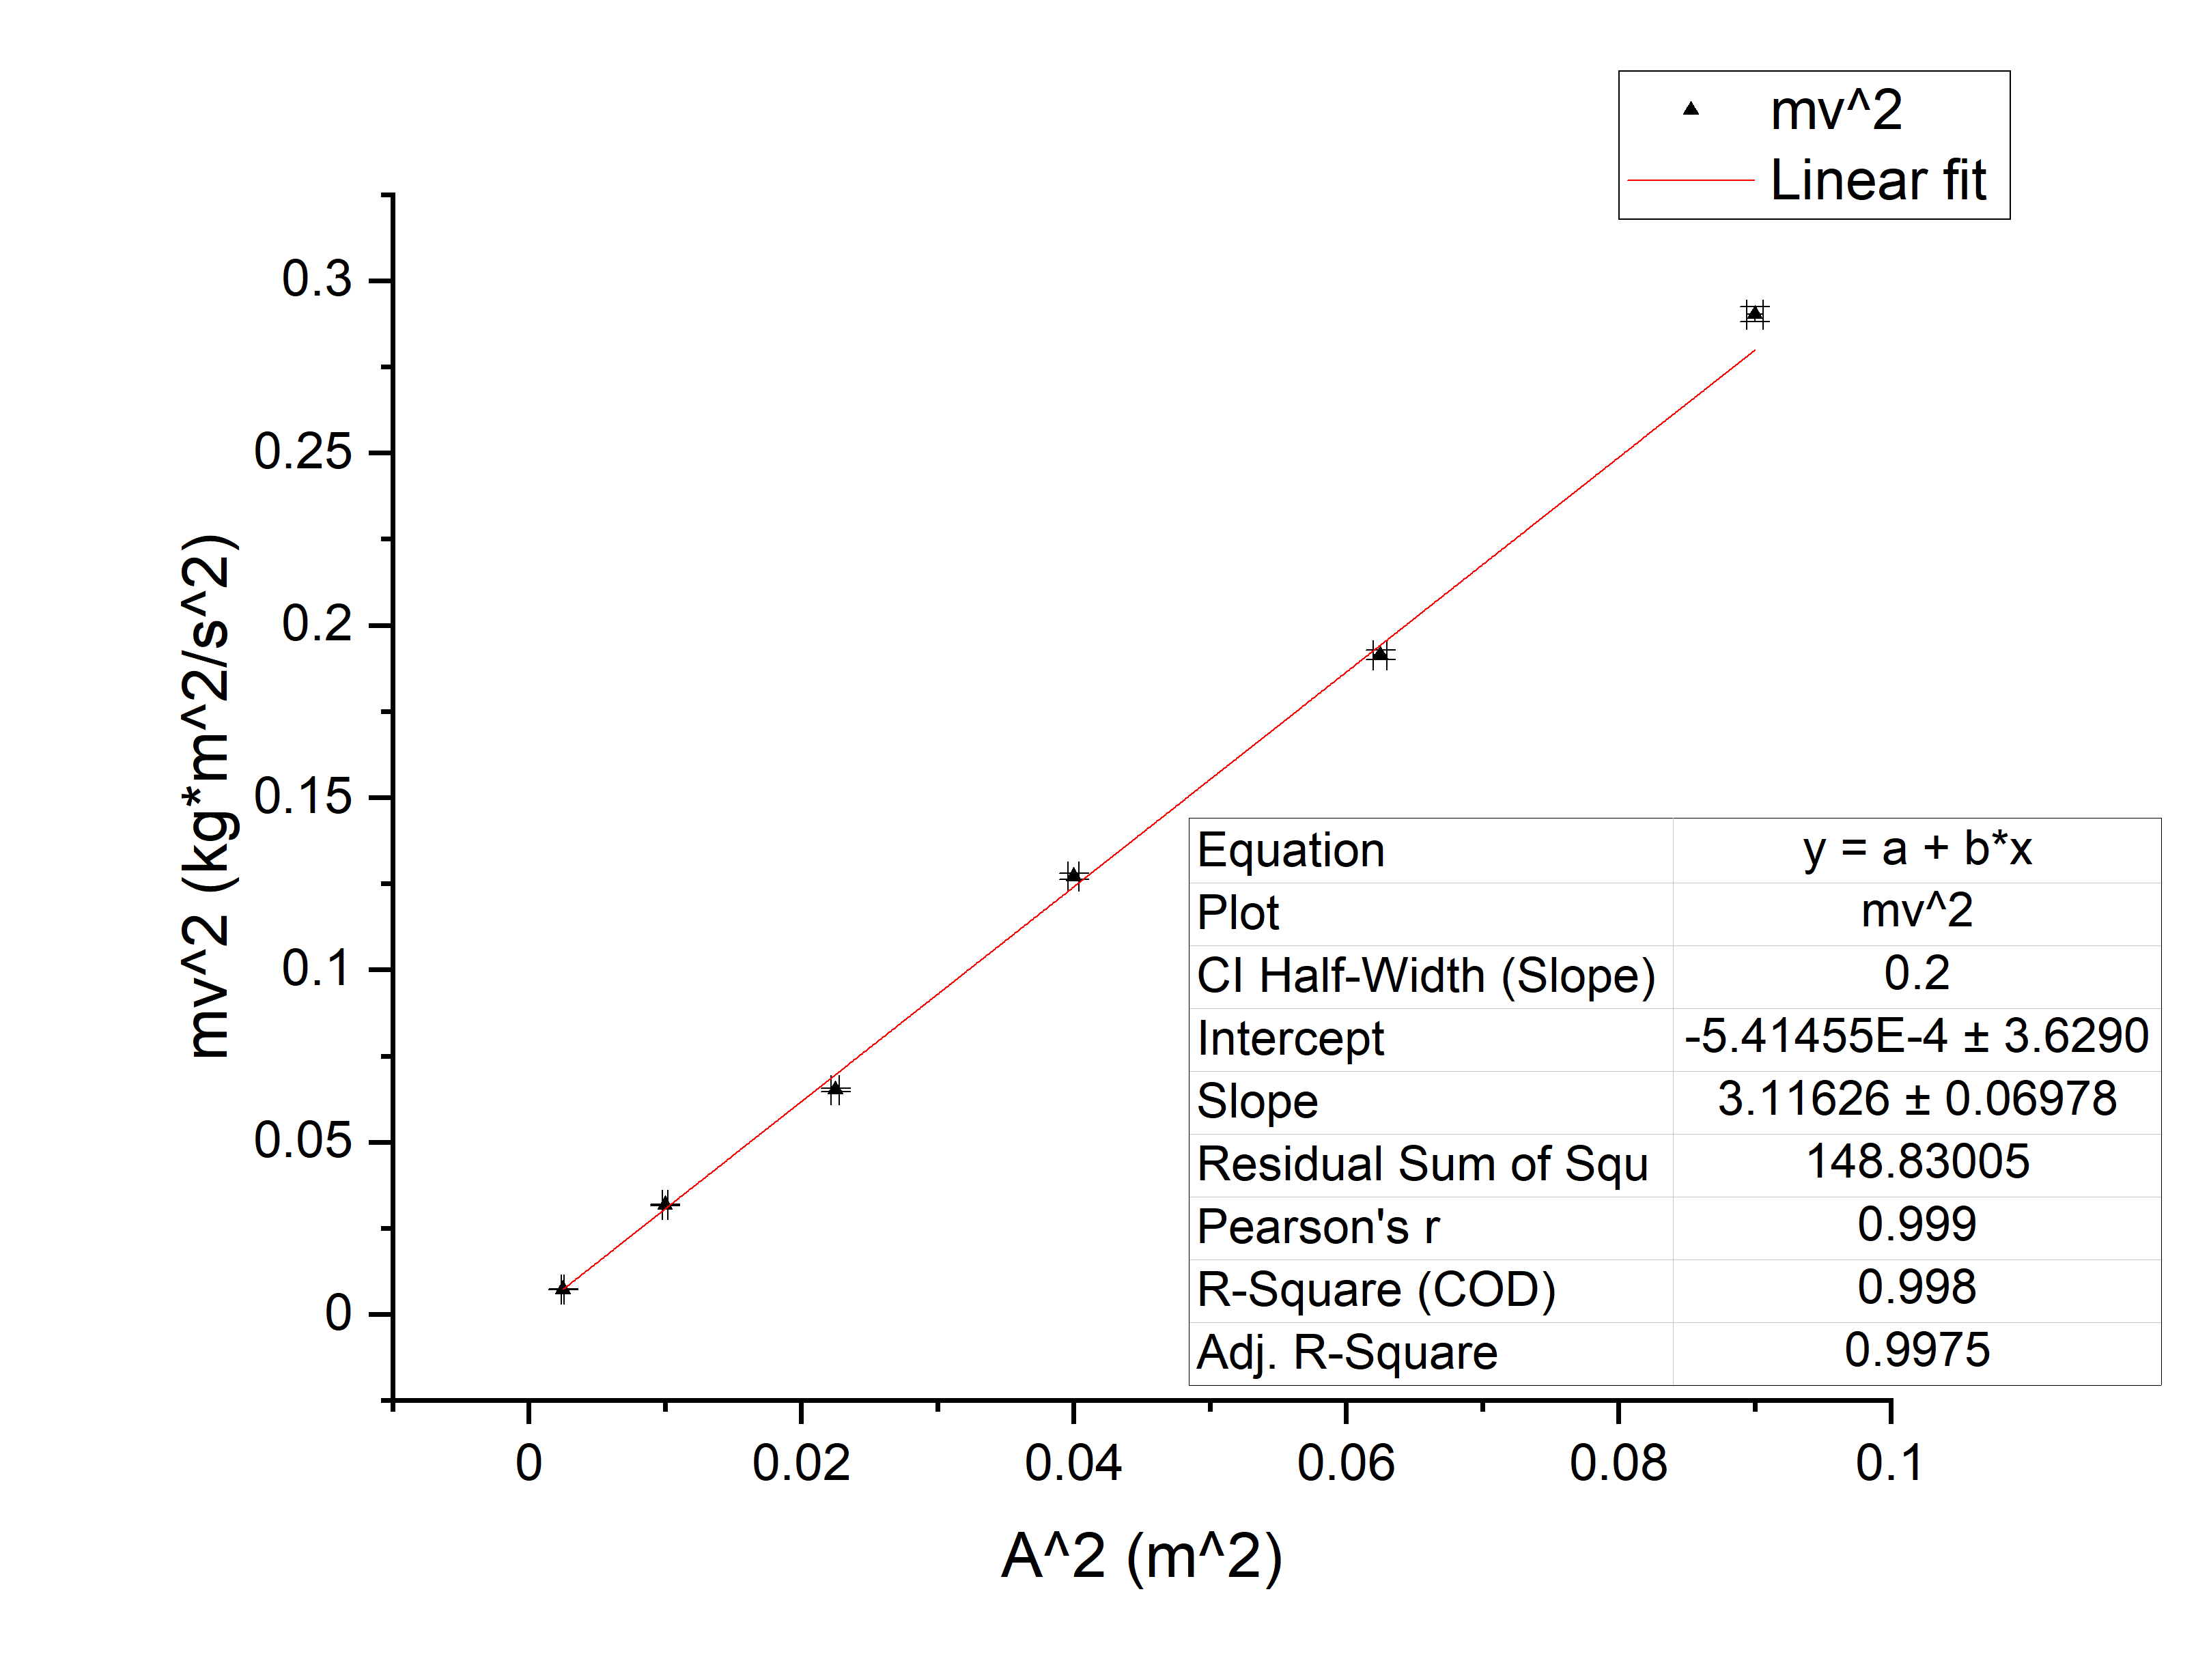
\includegraphics[scale=0.35]{mv2A2.png}
    \caption{$mv^2$ vs. $A^2$}
    \label{mva}
\end{figure}
\qquad Read from the graph we can get the value of the slope to be $3.1\pm 0.2[kg/s^2]$, Recall equation \ref{vmaequ} so that the theoretical value of the slope should be $k_1+k_2=3.32\pm 0.04[kg/s^2]$. The relative error is $3.3\%$, so the two values are relatively close.
\section{Conclusions and Discussion}
\subsection{Conclusions and Error Analyze}
\subsubsection{Measuring Spring Constant}
\qquad In this experiment, we read two spring constants from the graph. 

\begin{center}
    $k_1=1.66\pm 0.03[N/m] $, with relative uncertainty $1.81\%$\\
    $k_2=1.66\pm 0.03[N/m] $, with relative uncertainty $1.81\%$
\end{center}
\qquad The relative uncertainty is very small and from the fitting stastic we can see that Adj. R-square are 0.99978 and 0.99985 respectively, which are very close to 1, these prove that the fitting is efficient. However there may be some error here because in this experiment, we read the caliper manually and the spring is always oscillating slightly so that the value we read isn't that exact.
\subsubsection{Analyzing the Relation Between T and M}
\qquad Before we do the experiment, we know that the theoretical relationship of T and M is $$\frac{T^2}{M}=4\pi^2\cdot \frac{1}{k_1+k_2}$$
we get 3 values from graphs which are $11.795\pm 0.015,\  11.826\pm 0.030,\  11.82\pm 0.04 \ [s^2/kg]$ and calculate the theoretical value to be $11.9\pm 0.15[s^2/kg]$, the three relative error are all smaller than $1\%$, and the R-squre of fitting is extremely close to 1, which means the fitting is very ideal, so that we can say that T and M follows the expected relation.\par
\quad What may cause error here is 1. when we release the object, there may be an initial speed or resist the motion at the beginning 2. Although we use air track to eliminate air resistance, it does have some influence, which may affect the period.
\subsubsection{Analyzing the Relation Between Period T and Amplitude A}
\qquad From the figure, we can read that the correlation coefficient $\gamma=0.25<<1$ and the Adj. R-Square=-0.17<0, which shows that T and A don't have obvious relation. And the error is similar to the error in 5.2.
\subsubsection{Analyzing the Relation Between Maximum Speed and Amplitude}
\qquad From the figure we get $$k=3.1\pm 0.2[kg/s^2]$$. \quad $\ $Our theoretical value of the spring constant here is $$k_1+k_2=3.32\pm 0.04[kg/s^2]$$ and this gives the relative error to be $3.3\%$
\par $\ \ $What may cause error here except the reasons mentioned above in 5.2 and 5.3. It's also worth noticing that the value of v is calculated from several measured data. The complex calculation may also increase error.
\subsection{Suggestions}
\qquad For part 1 (measurement of spring constant), maybe we can use some electronic device to make the measurement more precise rather than read it manually. And for part 2,3,4, a release system can be used to ensure that when the object is released, no initial speed or resistance is forced on it.

%----------------------------------------------------------------------------------------
%	SECTION 7
%----------------------------------------------------------------------------------------
\section{Reference}
Qin Tian, Zheng Huan, Li Yingyu, Li Tiantian, Mateusz Krzyzosiak, Vp141, Exercise 3, Simple Harmonic Motion:
Oscillations in Mechanical Systems

%----------------------------------------------------------------------------------------
%	DATASHEET
%----------------------------------------------------------------------------------------

\section*{A Uncertainty Analysis}
\subsection*{A.1 Uncertainty in Measurement of Spring Constant}
For the measurement of the spring constant, the uncertainty of mg is calculated as follow. Since m is get directly from measurement, $\mu_m=0.01g=0.01\times 10^{-3}kg$
\begin{equation*}
    \mu_{mg}=\mu_m\cdot g=0.01\times 10^{-3}kg\times 9.794 m/s^2=9.794\times 10^{-5}N=0.0001N
\end{equation*}
And the uncertainty for all L is: 
\begin{equation*}
    \mu_L=0.02\times 10^{-3}m=2\times 10^{-5}m
\end{equation*}
Since we are using $\Delta L=L_x-L_0$, the uncertainty can be calculated from:
\begin{equation*}
    \mu_{\Delta_L}=\sqrt{\mu_L^2\times 2}=\sqrt{0.00002^2\times 2}=0.00003m
\end{equation*}
The uncertainty for the spring constant k can be read from the CI Half-Wdith of $mg-L$ line, which was calculated in the fitting procedure, which are respectively:
\\
\begin{equation*}
    \mu_{k_1}=0.03[N/kg]
\end{equation*}
\begin{equation*}
    \mu_{k_2}= 0.03[N/kg]
\end{equation*}

\subsection*{A.2 Uncertainty in Analyzing the Relation Between T and M}
    \qquad The uncertainty of 10T is given as 0.0001s, so that the uncertainty of T is 0.00001s. And then we can use that to calculate the uncertainty of T square (Table \ref{uncertainty of Tsquare}):
    \begin{equation}
        \mu_{T^2}=\left |\frac{dT^2}{dT}  \right |\cdot \mu_T=2T\cdot \mu_T
        \nonumber
    \end{equation}
    \qquad For example: for M1, horizontal, we have:
    \begin{equation*}
        \mu_{T^2}=2\times 1.24349s\times 0.00001s=0.00002s^2
    \end{equation*}
    \begin{table}[h]
        \centering
        \begin{tabular}{|c|c||c|c||c|c|}\hline
        \multicolumn{6}{|c|}{\textbf{Uncertainty of $T^2$[$s^2$]}}\\\hline 
        \multicolumn{2}{|c||}{horizontal}&\multicolumn{2}{c||}{incline 1}&\multicolumn{2}{c|}{incline 2}\\\hline
        $m_1$&0.00002 &$m_1$& 0.00002 & $m_1$&0.00002 \\\hline
        $m_2$&0.00003 & $m_2$&0.00003 & $m_2$&0.00003 \\\hline
        $m_3$&0.00003 &$m_3$& 0.00003 & $m_3$&0.00003 \\\hline
        $m_4$&0.00003 & $m_4$&0.00003 & $m_4$&0.00003 \\\hline
        $m_5$&0.00003 & $m_5$&0.00003 & $m_5$&0.00003 \\\hline
        $m_6$&0.00003 & $m_6$&0.00003 & $m_6$&0.00003\\\hline
        \end{tabular}
        \caption{}
        \label{uncertainty of Tsquare}
        \end{table}
\\\\
Also we need to calculate the uncertainty for m here since m is calculated by $m=M_0+m_{mass}=m_{obj}+m_{mass}+\frac{1}{3}m_{spr1\&2}$
\begin{equation*}
    \begin{split}
\mu_m&=\sqrt{\mu_{m_{obj}}^2+\mu_{m_{spr1\&2}}^2\times \frac{1}{3^2}+\mu_{m_{mass}}^2}\\ &=\sqrt{0.00001^2\times (1+1+\frac{1}{9})}\\ &=1.5\times 10^{-5}kg
    \end{split}
\end{equation*}
\qquad And recall that the uncertainty of the theoretical $T^2/m$ is:
\begin{equation*}
    \frac{T^2}{m}=\frac{4\pi^2}{k_1+k_2}
\end{equation*}
\newpage
Therefore the uncertainty of the theoretical $T^2/m$ is:
\begin{equation*}
    \begin{split}
        \mu_{T^2/m}&=\sqrt{\left(\frac{\partial \frac{4\pi^2}{k_1+k_2}}{\partial k_1}\right)^2\cdot \mu_{k_1}^2+\left(\frac{\partial \frac{4\pi^2}{k_1+k_2}}{\partial k_2}\right)^2\cdot \mu_{k_2}^2}\\
        &=\sqrt{\left(\frac{-4\pi^2}{(k_1+k_2)^2}\right)^2\cdot \mu_{k_1}^2+\left(\frac{-4\pi^2}{(k_1+k_2)^2}\right)^2\cdot \mu_{k_2}^2}\\
        &=\sqrt{\left(\frac{-4\pi^2}{(1.66+1.66)^2}\right)^2\cdot 0.03^2+\left(\frac{-4\pi^2}{(1.66+1.66)^2}\right)^2\cdot 0.03^2}\\
        &=0.15[s^2/kg]
    \end{split}
\end{equation*}
\subsection*{A.3 Uncertainty of Analyzing the Relation Between Period T and Amplitude A}
\qquad In this part, the amplitude has the uncertainty of 0.1cm and $T_{10}$ has the uncertainty of 0.0001s, so the uncertainty of T is 0.00001s. The uncertainty of the relationship of T and A is given by the fitting.
\subsection*{A.4 Uncertainty of Analyzing the Relation Between Maximum Speed and Amplitude A}
\subsubsection*{A.4.1 $\mathbf{\Delta x:\ x_{in}\ and\ x_{out}}$}
\qquad The type-B uncertainty for $x_{in}$ is $\Delta x_{in} = 0.02mm$. To find the type-A uncertainty, we first find the standard deviation.
\begin{equation*}
    s_{x_{in}}=\sqrt{\frac{1}{n-1}\left( \sum_{i=1}^nx_{in_i}-\overline{x}_{in} \right)^2}=\sqrt{\frac{1}{2}\left((4.42-4.44)^2+(4.44-4.44)^2+(4.46-4.44)^2\right)}=0.02[mm]
\end{equation*}
\qquad We have n=3, so the type-A uncertainty $\Delta_{x_{in_A}}$ is calculated as 
\begin{equation*}
    \Delta_{x_{in_A}}=\frac{t_{0.95}}{\sqrt{n}}s_{x_{in}}=2.48\times0.02=0.05[mm]
\end{equation*}
\qquad Hence the uncertainty for $x_{in}$ is given by 
\begin{equation*}
    \mu_{x_{in}}=\sqrt{\Delta_{x_{in_A}}^2+\Delta_{x_{in_B}}^2}=0.05[mm]
\end{equation*}
\qquad Hence $x_{in}$ is given by 
\begin{equation*}
    x_{in}=4.44\pm 0.05[mm]
\end{equation*}\\\par
$\ $ Similarly, we can calculate the uncertainty for $x_{out}$:\par
$\ $ The type-B uncertainty for $x_{out}$ is $\Delta x_{out} = 0.02mm$. To find the type-A uncertainty, we first find the standard deviation.
\begin{equation*}
    s_{x_{out}}=\sqrt{\frac{1}{n-1}\left( \sum_{i=1}^nx_{out_i}-\overline{x}_{out} \right)^2}=\sqrt{\frac{1}{2}\left((15.56-15.56)^2+(15.56-15.54)^2+(15.56-15.58)^2\right)}=0.02[mm]
\end{equation*}
\qquad We have n=3, so the type-A uncertainty $\Delta_{x_{out_A}}$ is calculated as 
\begin{equation*}
    \Delta_{x_{out_A}}=\frac{t_{0.95}}{\sqrt{n}}s_{x_{out}}=2.48\times0.02=0.05[mm]
\end{equation*}

\par$\ $ Hence the uncertainty for $x_{out}$ is given by 
\begin{equation*}
    \mu_{x_{out}}=\sqrt{\Delta_{x_{out_A}}^2+\Delta_{x_{out_B}}^2}=0.05[mm]
\end{equation*}
\newpage
 Hence $x_{out}$ is given by 
\begin{equation*}
    x_{out}=15.56\pm 0.05[mm]
\end{equation*}

Then we proceed to calculate the uncertainty for $\Delta x$, Recall that:
\begin{equation}
    \Delta x=\frac{\overline x_{in}+\overline x_{out}}{2}
    \nonumber
\end{equation}
\qquad So the uncertainty of $\Delta x$ can be calculated by: 
\begin{equation*}
    \begin{split}
    \mu_{\Delta_x}&=\sqrt{\frac{1}{2^2}\cdot \mu_{x_{in}}^2+\frac{1}{2^2}\cdot \mu_{x_{out}}^2}\\
    &=\sqrt{\frac{1}{4}\times 0.05^2+\frac{1}{4}\times 0.05^2}\\
    &=0.0350725=0.04[mm]
    \end{split}
\end{equation*}
\qquad Hence $\Delta x$ is given by $$\Delta x= 10.0\pm 0.04[mm]=0.01\pm0.00004[m]$$\\


\subsubsection*{A.4.2 $\mathbf{v:\ \Delta x\ and\ \Delta t}$}
\qquad Recall that $$v=\frac{\Delta x}{\Delta t}$$
\qquad So that we can calculate the uncertainty for v by:
\begin{equation*}
    \begin{split}
        \mu_v&=\sqrt{\left(\frac{\partial v}{\partial \Delta t}\right)^2\cdot (\mu_{\Delta t})^2+\left(\frac{\partial v}{\partial \Delta x}\right)^2\cdot (\mu_{\Delta x})^2}\\
        &=\sqrt{\left(\frac{1}{\Delta t}\right)^2\cdot (\mu_{\Delta x})^2+\left(\frac{\Delta x}{\Delta t^2}\right)^2\cdot (\mu_{\Delta t})^2}
    \end{split}
\end{equation*}
\qquad For example, for the set of data: $A=0.050\pm0.001[m]\ \ \Delta t=0.04771\pm0.00001[s]$
\begin{equation*}
    \begin{split}
        \mu_v&=\sqrt{\left(\frac{1}{\Delta t}\right)^2\cdot (\mu_{\Delta x})^2+\left(\frac{\Delta x}{\Delta t^2}\right)^2\cdot (\mu_{\Delta t})^2}\\
        &=\sqrt{\frac{1}{0.04771^2}\times 0.0000350725^2+\left(\frac{0.01}{0.04771^2}\right)^2\times 0.00001^2}\\
        &=0.0007[m/s]
    \end{split}
\end{equation*}
\qquad Similarly, the uncertainty of other sets of data are presented in Table \ref{uncertainty of mu v}
\\
\begin{table}[h]
    \centering
    \begin{tabular}{|c|c|}\hline
    $A[m]\pm 0.001[m]$& $\mu_v[m/s]$\\\hline
    0.050 & 0.0007 \\
    0.100 & 0.0016 \\
    0.150 & 0.002  \\
    0.200 & 0.003  \\
    0.250 & 0.004  \\
    0.300 & 0.005 \\\hline
    \end{tabular}
    \caption{Uncertainty for v}
    \label{uncertainty of mu v}
\end{table}
\newpage
\subsubsection*{A.4.3 $\mathbf{v_{max}, A\ and\ m}$}
\qquad Recall that $$k=\frac{mv_{max}^2}{A^2}$$
\qquad so that for plotting we need to calculate the uncertainty for $mv_{max}^2$ and the uncertainty for $A^2$\par
$\ $To start with, we first calculate the uncertainty for m which is the same as the uncertainty of m in A.2
$$\mu_m=0.000015[kg]$$
\begin{enumerate}
    \item $\mathbf{\mu_{mv_{max}^2}}$
    \\
    \\ To be simplified, we denote $v_{max}$ by $v$ in the following calculation.\\
    \begin{equation*}
        \begin{split}
        \mu_{mv^2}&=\sqrt{\left(\frac{\partial mv^2}{\partial m}\right)^2\cdot \mu_m^2+\left(\frac{\partial mv^2}{\partial v}\right)^2\cdot \mu_v^2}\\
        &=\sqrt{\left(v^2\right)^2\cdot \mu_m^2+\left(2mv\right)^2\cdot \mu_v^2}
        \end{split}
    \end{equation*}
    For example for the set of data :
    \begin{table}[h]
        \centering
        \begin{tabular}{cccc}
        $v$  & $\mu_v$ & $m$     & $\mu_m$ \\\hline
        0.21 & 0.0007  & 0.16407 & 0.000015
        \end{tabular}
        \end{table}\par
    We have: 
    \begin{equation*}
        \begin{split}
            \mu_{mv^2}&=\sqrt{\left(v^2\right)^2\cdot \mu_m^2+\left(2mv\right)^2\cdot \mu_v^2}\\
            &=\sqrt{(0.21^2)^2\times 0.000015^2+(2\times 0.16407\times 0.21)^2\times 0.0007^2}\\
            &=0.00005[kg\cdot m^2/s^2]
        \end{split}
    \end{equation*}
     Similarly, the uncertainty of all data sets are shown in table \ref{Uncertainty for mv2}:
    \begin{table}[h]
        \centering
        \begin{tabular}{c|c|c|c|c}
            $v$  & $\mu_v$ & $m$     & $\mu_m$& $\mu_{mv^2}$ \\\hline  
        0.21 & 0.0007 & 0.16407 & 0.00001 & 0.00005 \\
        0.44 & 0.0016 & 0.16407 & 0.00001 & 0.0002  \\
        0.63 & 0.0023 & 0.16407 & 0.00001 & 0.0005  \\
        0.88 & 0.0032 & 0.16407 & 0.00001 & 0.0009  \\
        1.08 & 0.0040 & 0.16407 & 0.00001 & 0.0014  \\
        1.33 & 0.0050 & 0.16407 & 0.00001 & 0.002  
        \end{tabular}
        \caption{Uncertainty for $mv^2$}
        \label{Uncertainty for mv2}
        \end{table}
    \item $\mathbf{\mu_{A^2}}$\\
    $$\mu_{A^2}=\left| \frac{dA^2}{dA}\right|\cdot \mu_A=2A\cdot \mu_A$$
    For example: for A=0.05m we have: $\mu_A=2\times 0.05\times 0.001=0.0001[m^2]$
    And similarly the uncertainty for all $A^2$ are shown in table following (Table \ref{unceratinya2}):
   \begin{table}[H]
    \centering
        \begin{tabular}{c|c}
          A[m]   &   $\mu_{A^2}[m^2]$     \\\hline
        0.0500 & 0.0001 \\
        0.1000  & 0.0002 \\
        0.1500 & 0.0003 \\
        0.2000  & 0.0004 \\
        0.2500 & 0.0005 \\
        0.3000  & 0.0006\\
        \end{tabular}
        \caption{Uncertainty for $A^2$}
        \label{unceratinya2}
    \end{table}
\end{enumerate}
\newpage
\subsubsection*{A.4.4 k}
\qquad From the figure of $mv_{max}^2\ vs.\ A^2$, we can directly read the uncertainty of k.\par
$\ $And for the theoretical value of k, we get it from $k_1+k_2$, so the uncertainty for this is 
\begin{equation*}
    \begin{split}
    \mu_k&=\sqrt{\mu_{k_1}^2+\mu_{k_2}^2}\\
    &=\sqrt{0.03^2+0.03^2}\\
    &=0.04[kg/s^2]
    \end{split}
\end{equation*}


\newpage
\section*{B Data Sheet}
\begin{figure}[H]
    \centering
    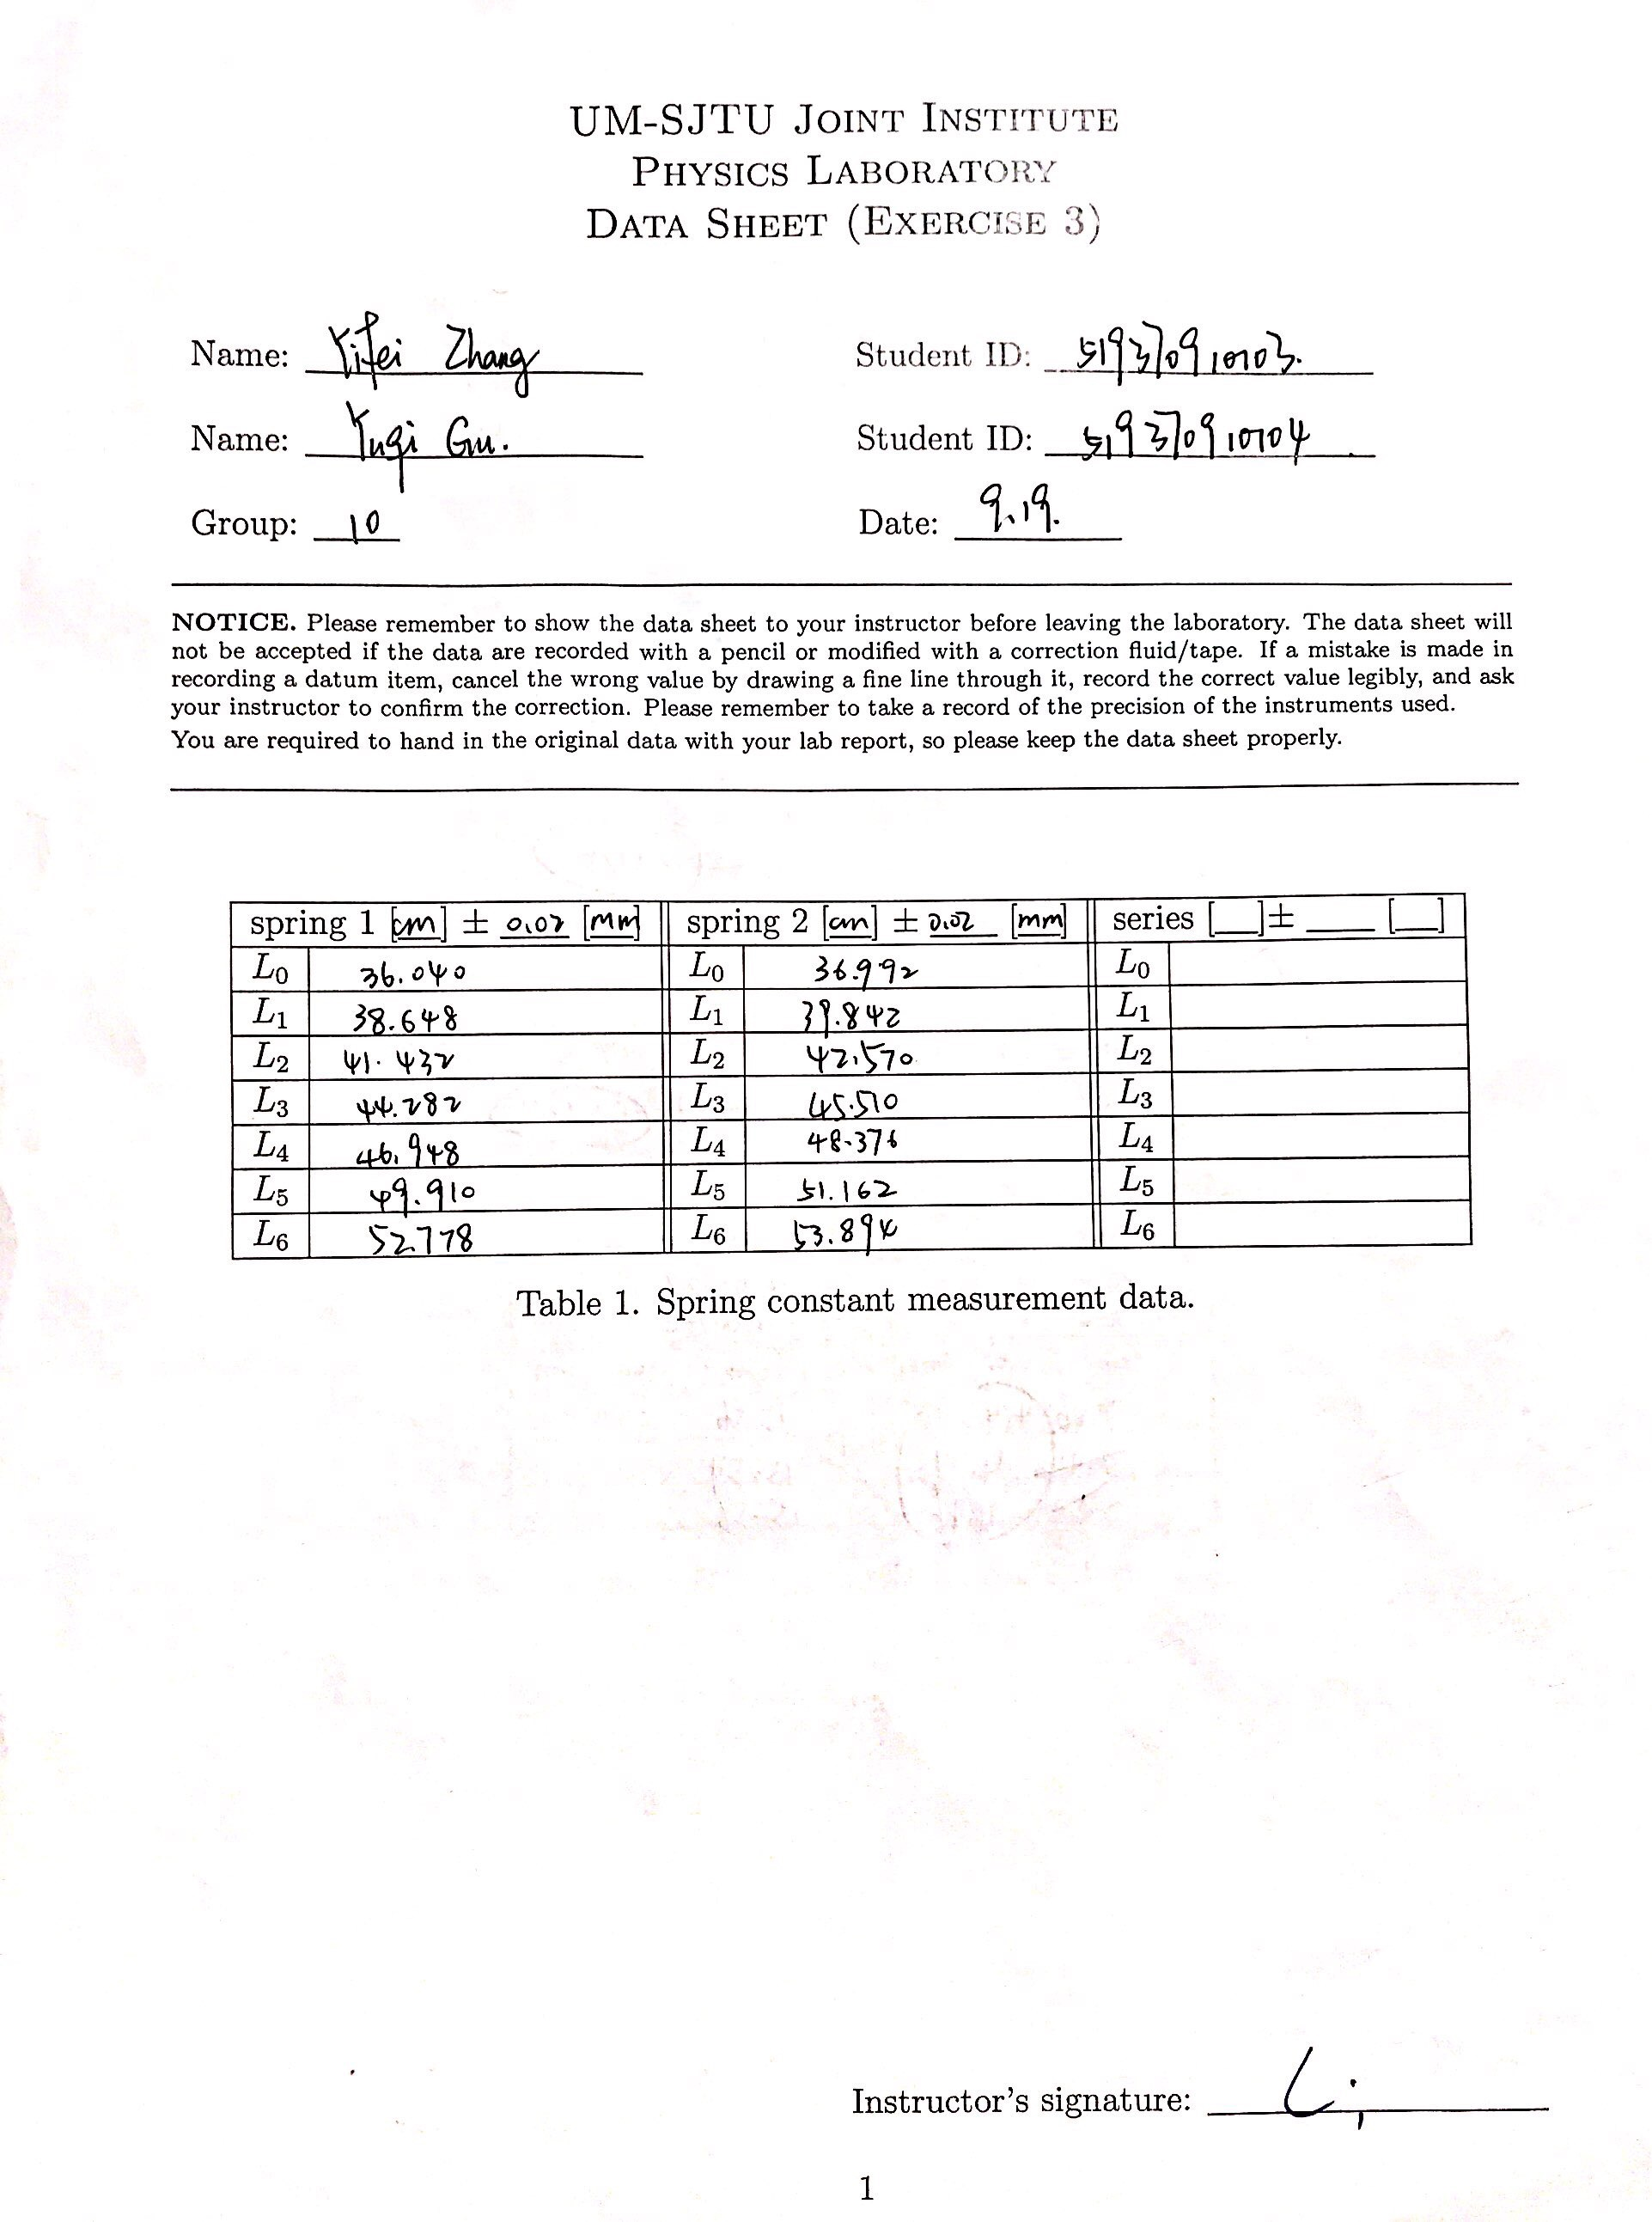
\includegraphics[scale=0.3]{data1.jpeg}

\end{figure}
\begin{figure}[H]
    \centering
    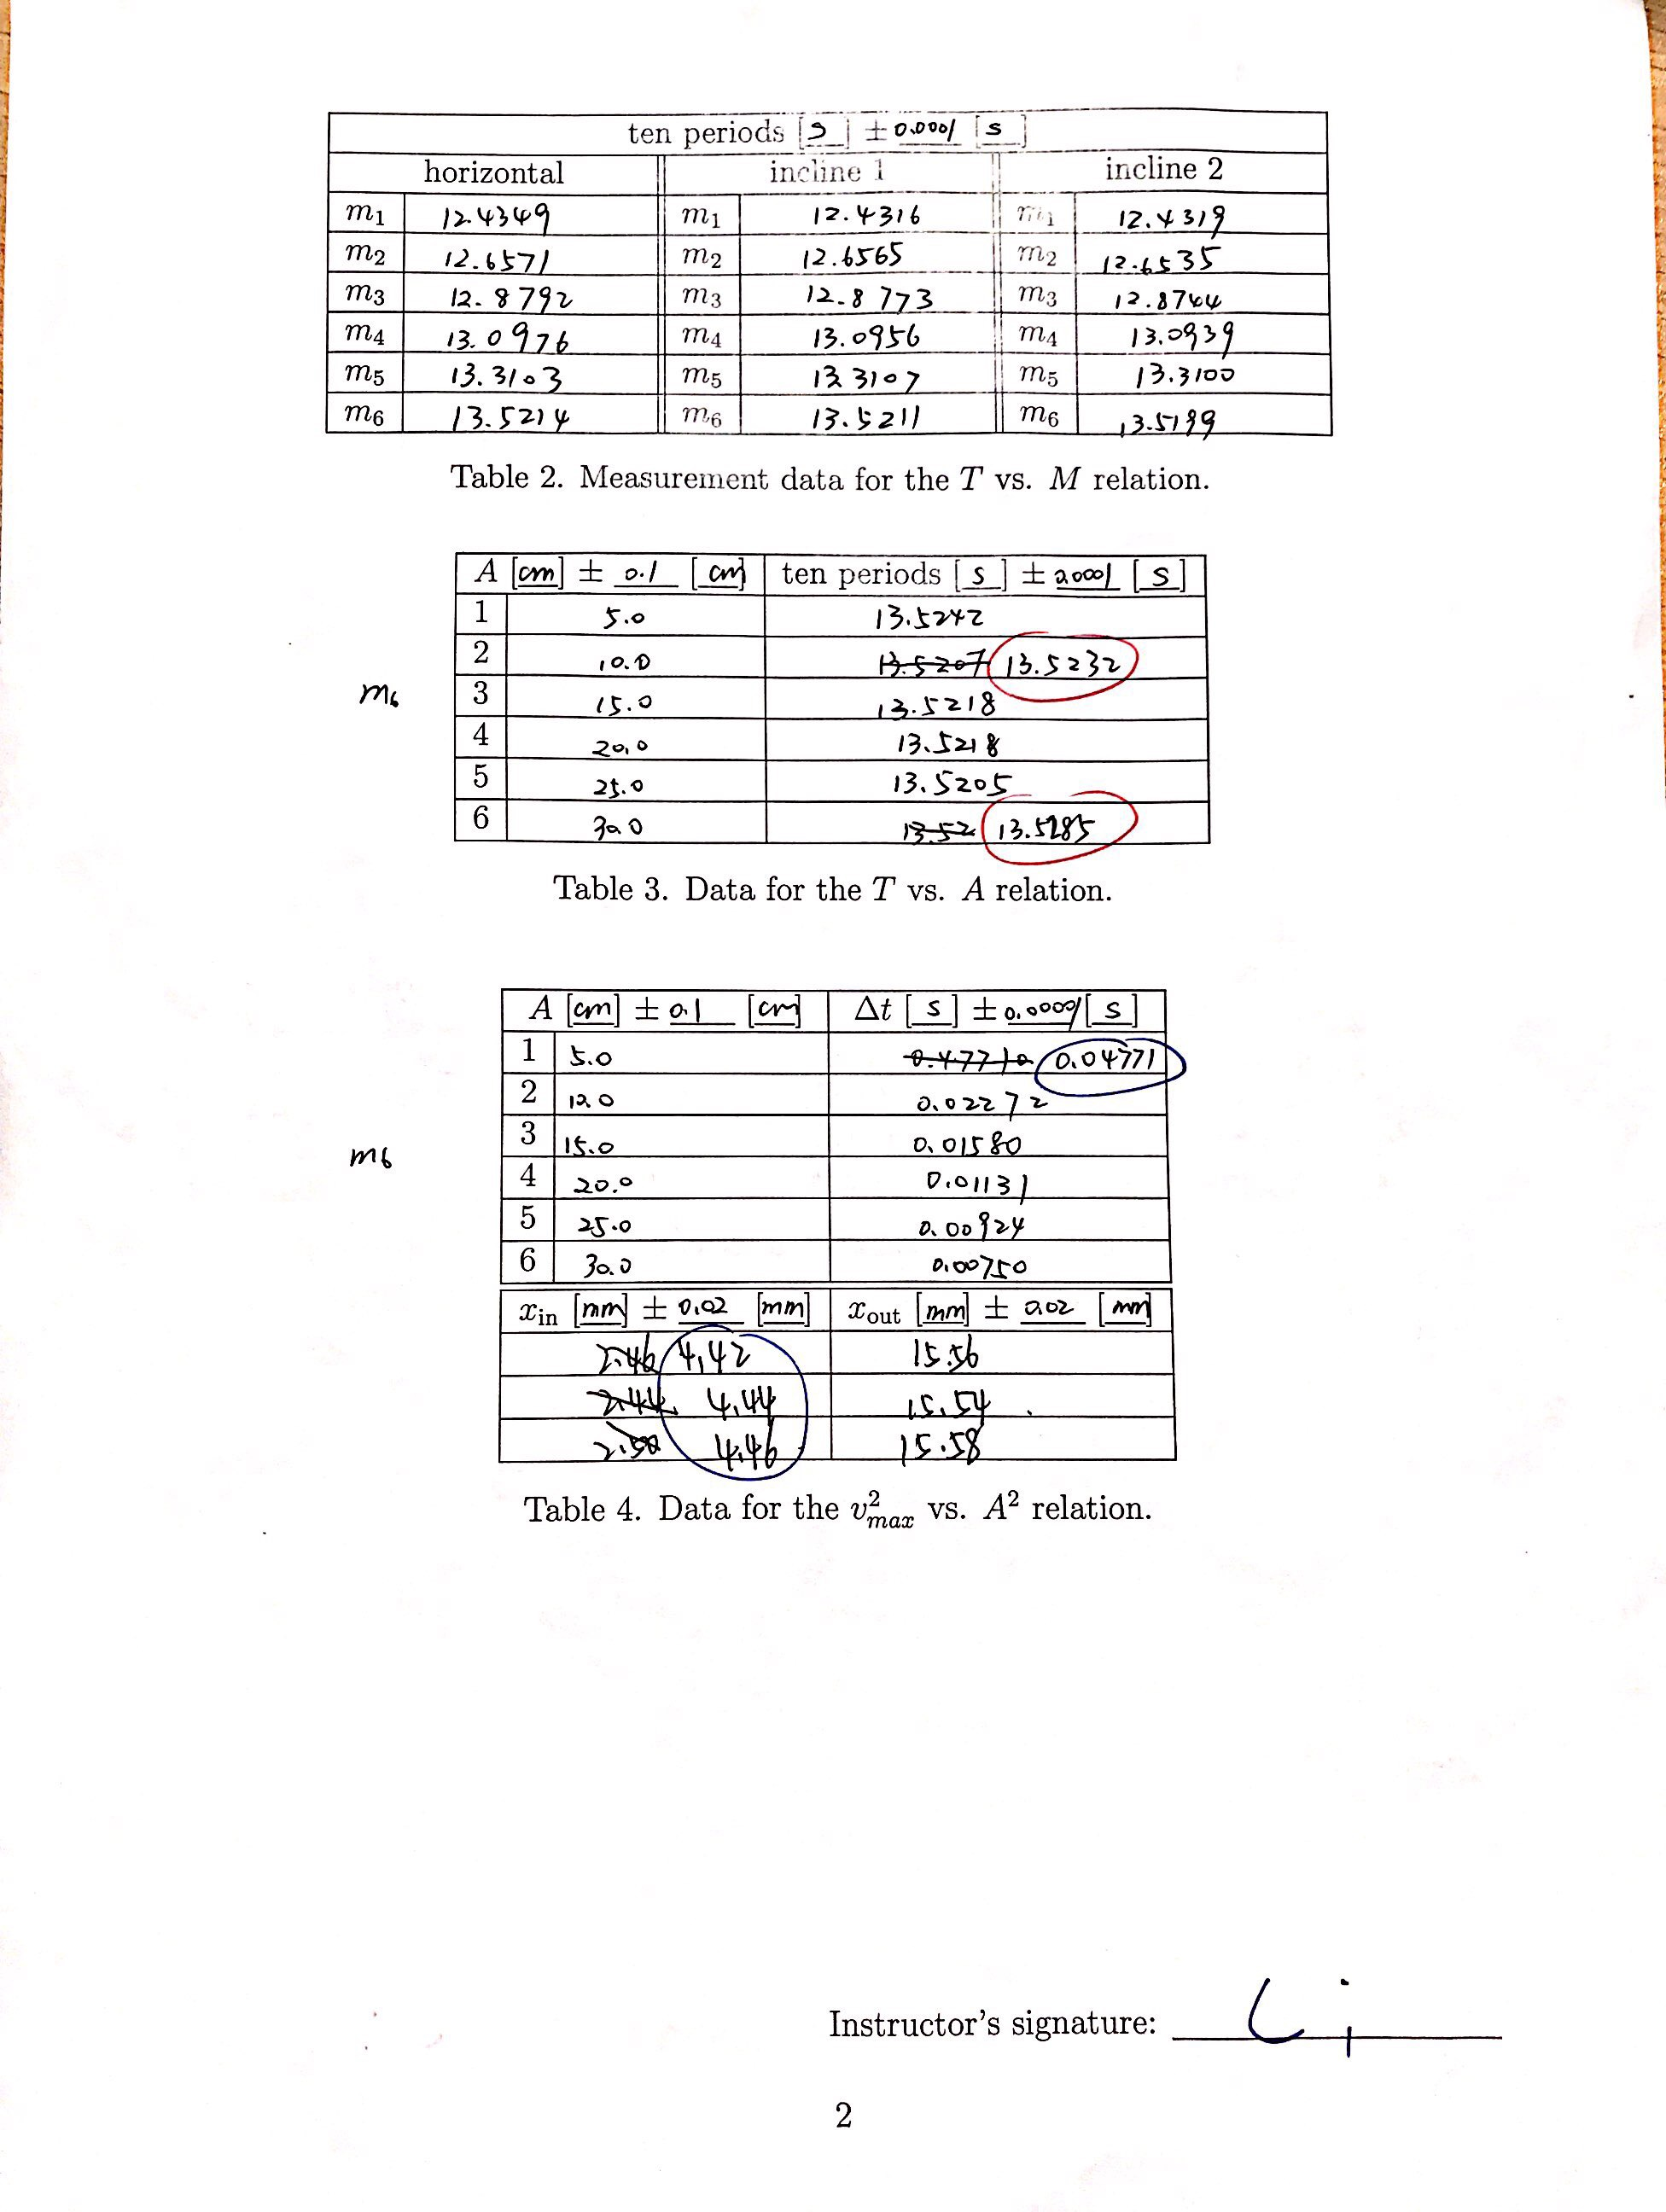
\includegraphics[scale=0.3]{data2.jpeg}

\end{figure}
\begin{figure}[H]
    \centering
    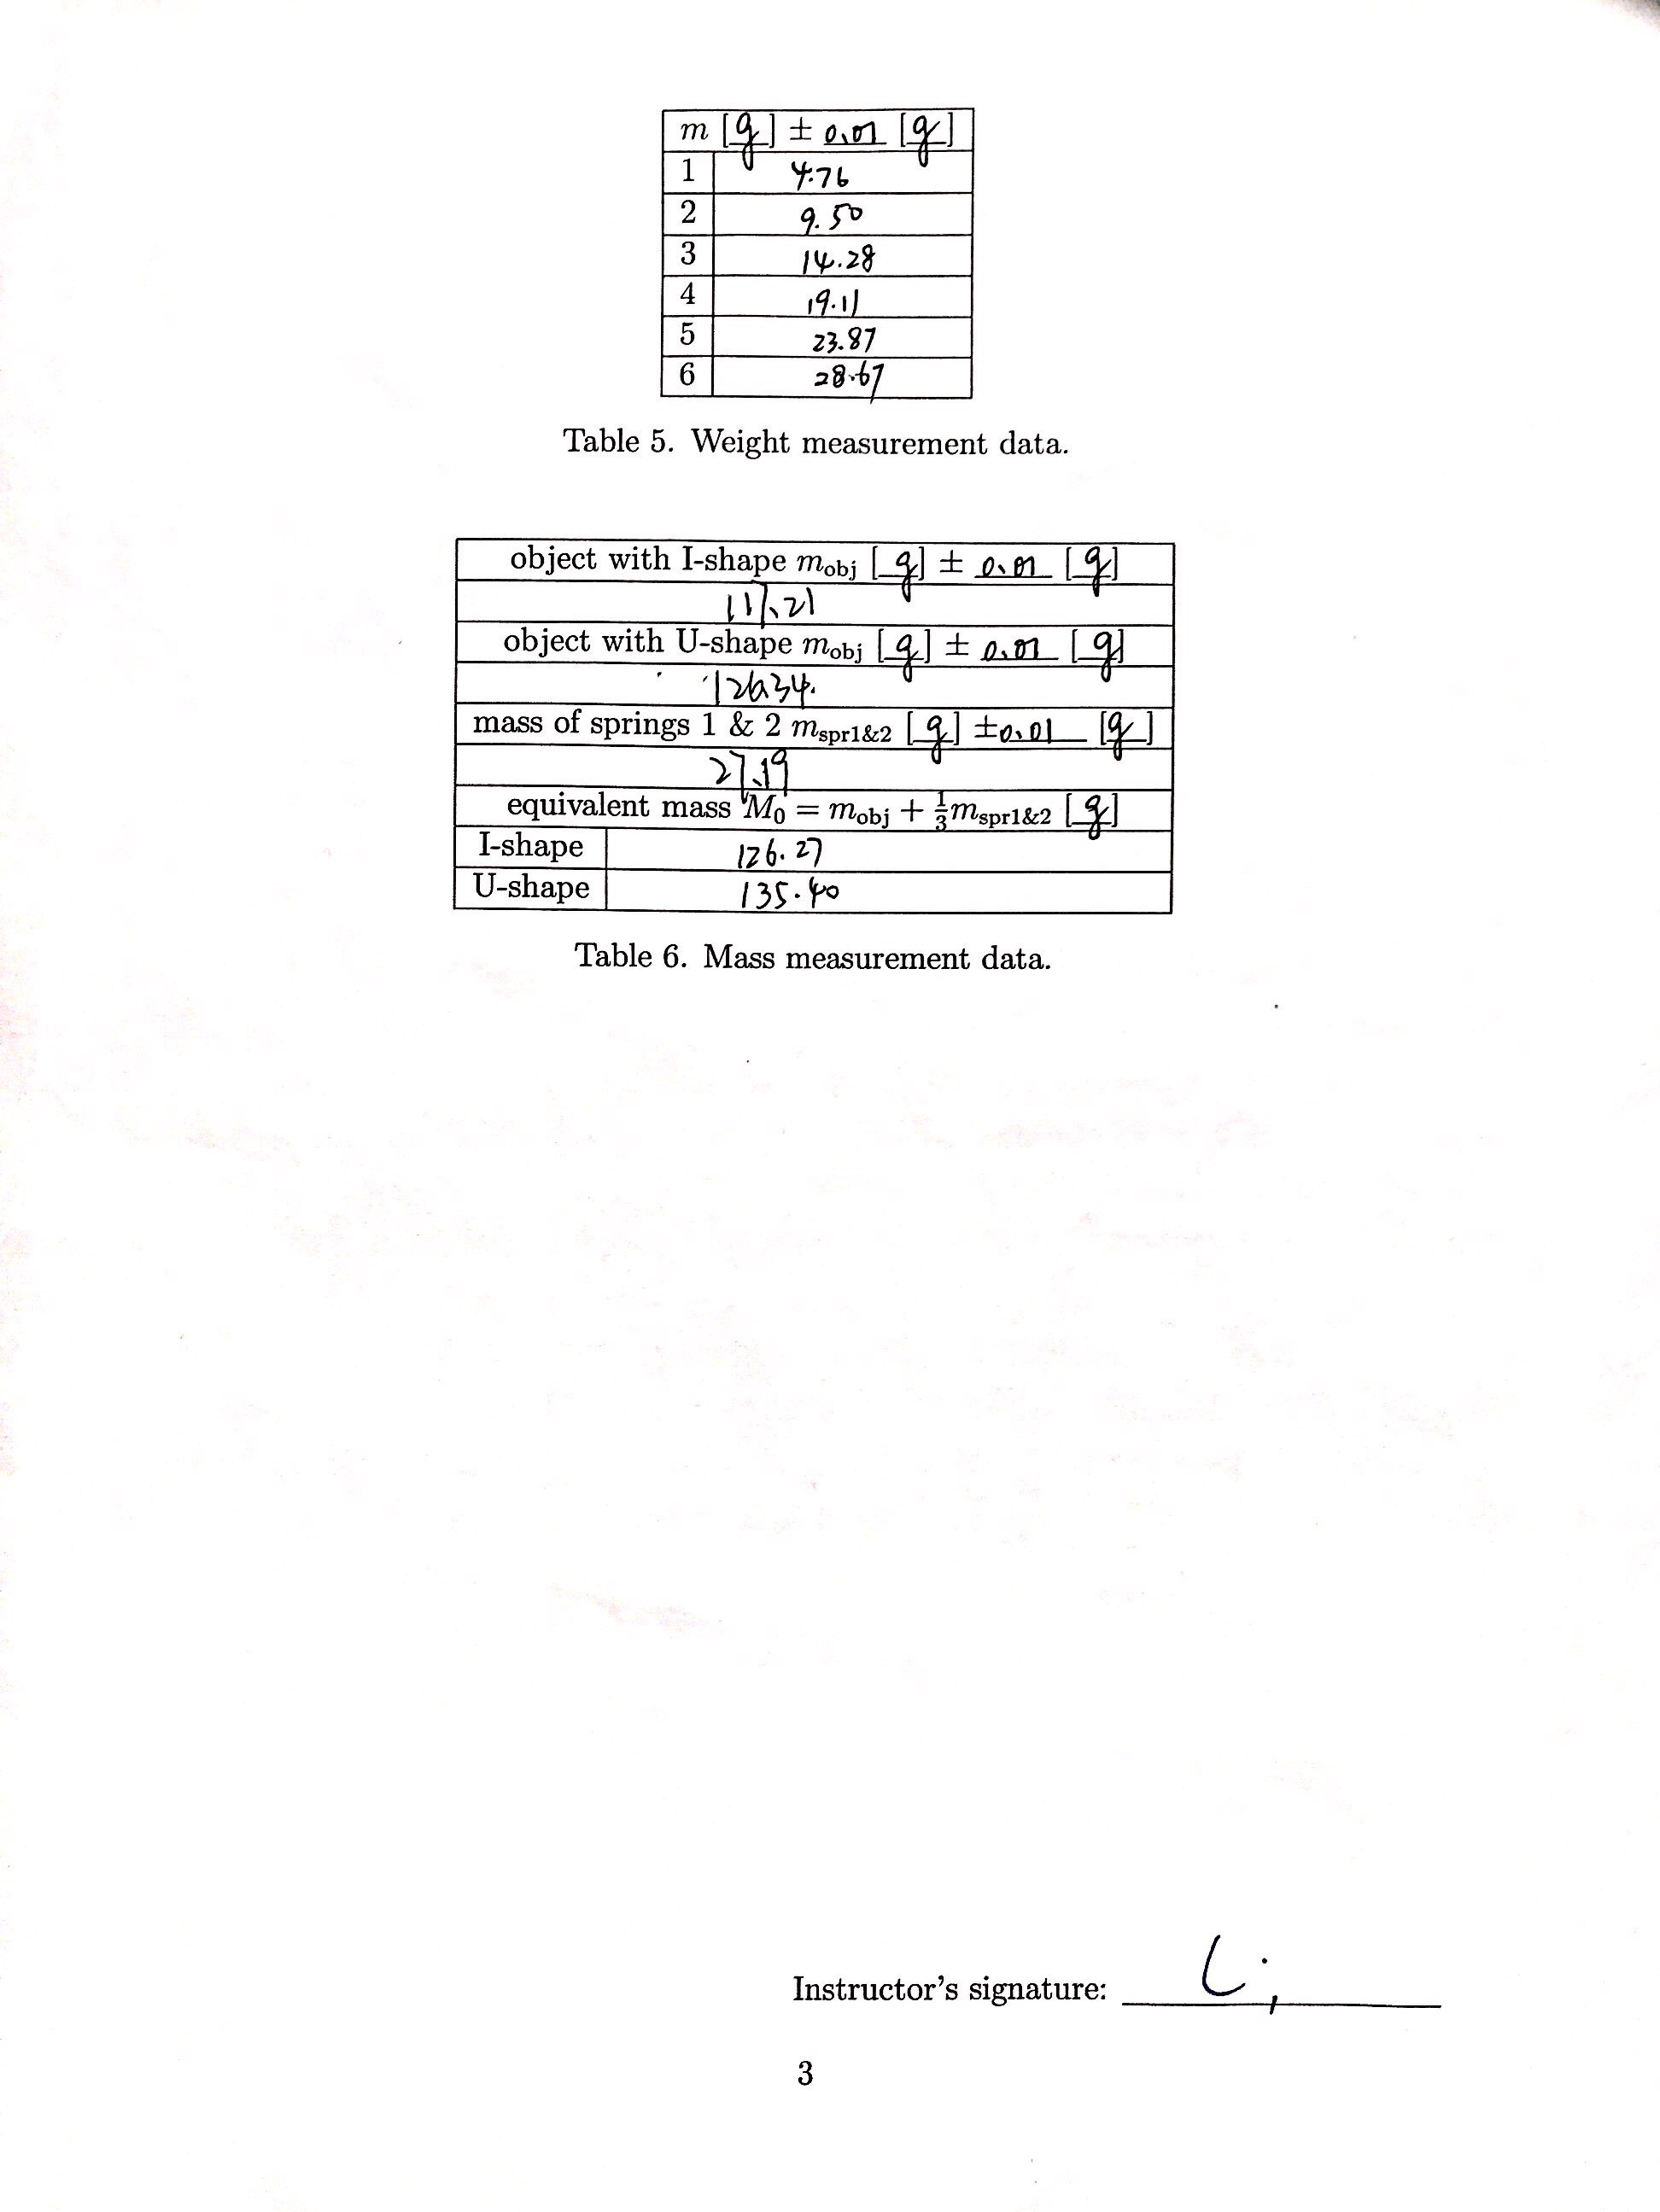
\includegraphics[scale=0.3]{data3.jpeg}

\end{figure}
\section*{C Supporting Information}
\begin{table}[h]
    \centering
    \begin{tabular}{|c|c||c|c|}\hline
    \multicolumn{2}{|c||}{spring 1[m]$\pm 0.00002[m]$}&\multicolumn{2}{c|}{spring 2[m]$\pm 0.00002[m]$}\\\hline
    $L_0$&   0.36040     &   $L_0$   &0.36992\\\hline
    $L_1$&0.38648&$L_1$& 0.39842\\\hline
    $L_2$&0.41432 & $L_2$&0.42570 \\\hline
    $L_3$& 0.44282  &$L_3$& 0.45510 \\\hline
    $L_4$&0.46948 & $L_4$&0.48376  \\\hline
    $L_5$&0.49910 & $L_5$&0.51162\\\hline
    $L_6$&0.52778 & $L_6$&0.53894 \\\hline
    \end{tabular}
    \caption{measurement data for spring constant}
    \label{measurespringconstant}
\end{table}

\begin{table}[h]
    \centering
    \begin{tabular}{|c|c||c|c|}\hline
    \multicolumn{2}{|c||}{spring 1[m]$\pm 0.00002[m]$}&\multicolumn{2}{c|}{spring 2[m]$\pm 0.00002[m]$}\\\hline
    
    $\Delta L_1$&0.02608&$\Delta L_1$& 0.02850\\\hline
    $\Delta L_2$&0.02784 & $\Delta L_2$&0.02728 \\\hline
    $\Delta L_3$& 0.02850  &$\Delta L_3$& 0.02940 \\\hline
    $\Delta L_4$&0.02666 & $\Delta L_4$&0.02866 \\\hline
    $\Delta L_5$&0.02962 & $\Delta L_5$&0.02786\\\hline
    $\Delta L_6$&0.02868 & $\Delta L_6$&0.02732 \\\hline
    \end{tabular}
    \caption{$\Delta L$}
    \label{deltal}
\end{table}
\begin{table}[h]
    \centering
    \begin{tabular}{|c|c|}\hline
        \multicolumn{2}{|c|}{$m[kg]\pm0.00001[kg]$}\\\hline
    1 & 0.00476 \\\hline
    2 & 0.00950 \\\hline
    3 & 0.01428 \\\hline
    4 & 0.01911 \\\hline
    5 & 0.02387 \\\hline
    6 & 0.02867\\\hline
    \end{tabular}
    \caption{mass of the masses}
    \label{massofthemasses}
\end{table}


        \begin{longtable}{|c|c|}
        \hline
        \multicolumn{2}{|c|}{$mg[N]\pm0.0001[N]$}\\\hline
        1 & 0.047 \\ \hline
        2 & 0.093 \\ \hline
        3 & 0.140 \\ \hline
        4 & 0.187 \\ \hline
        5 & 0.234 \\ \hline
        6 & 0.281 \\ \hline
        \caption{value of mg}
        \label{mg}
        \end{longtable}
        \begin{table}[H]
            \centering
            \begin{tabular}{|c|c|c|c|c|c|}
            \hline
            \multicolumn{6}{|c|}{$T\pm 0.00001[s]$}                                                            \\ \hline
            \multicolumn{2}{|c|}{horizontal} & \multicolumn{2}{c|}{incline 1} & \multicolumn{2}{c|}{incline 2} \\ \hline
            $m_1$          & 1.24349         & $m_1$         & 1.24316        & $m_1$         & 1.24319        \\ \hline
            $m_2$          & 1.26571         & $m_2$         & 1.26565        & $m_2$         & 1.26535        \\ \hline
            $m_3$          & 1.28792         & $m_3$         & 1.28773        & $m_3$         & 1.28744        \\ \hline
            $m_4$          & 1.30976         & $m_4$         & 1.30956        & $m_4$         & 1.30939        \\ \hline
            $m_5$          & 1.33103         & $m_5$         & 1.33107        & $m_5$         & 1.33100        \\ \hline
            $m_6$          & 1.35214         & $m_6$         & 1.35211        & $m_6$         & 1.35199        \\ \hline
            \end{tabular}
            \caption{Value for T in $T\ vs.\ M$ relation}
            \label{valuettm}
            \end{table}
        \begin{table}[H]
            \centering
            \begin{tabular}{|c|c|c|c|c|c|}
            \hline
            \multicolumn{6}{|c|}{$T^2[s^2]$}                                                                   \\ \hline
            \multicolumn{2}{|c|}{horizontal} & \multicolumn{2}{c|}{incline 1} & \multicolumn{2}{c|}{incline 2} \\ \hline
            $m_1$          & 1.54627         & $m_1$         & 1.54545        & $m_1$         & 1.54552        \\ \hline
            $m_2$          & 1.60202         & $m_2$         & 1.60187        & $m_2$         & 1.60111        \\ \hline
            $m_3$          & 1.65874         & $m_3$         & 1.65825        & $m_3$         & 1.65750        \\ \hline
            $m_4$          & 1.71547         & $m_4$         & 1.71495        & $m_4$         & 1.71450        \\ \hline
            $m_5$          & 1.77164         & $m_5$         & 1.77175        & $m_5$         & 1.77156        \\ \hline
            $m_6$          & 1.82828         & $m_6$         & 1.82820        & $m_6$         & 1.82788        \\ \hline
            \end{tabular}
            \caption{Value for $T^2$ in $T\ vs.\ M$ relation}
            \label{valueT2}
            \end{table}
            \begin{table}[H]
                \centering
                \begin{tabular}{|c|c|}
                \hline
                \multicolumn{2}{|c|}{$m_{all}[kg]\pm0.000015[kg]$} \\ \hline
                1                   & 0.13103                   \\ \hline
                2                   & 0.13577                   \\ \hline
                3                   & 0.14055                   \\ \hline
                4                   & 0.14538                   \\ \hline
                5                   & 0.15014                   \\ \hline
                6                   & 0.15494                   \\ \hline
                \end{tabular}
                \caption{equivalent mass of different masses with I-shape}
                \label{equivalent2}
                \end{table}

                    \begin{table}[H]
                        \centering
                        \begin{tabular}{|c|c|c|}
                        \hline
                        A[m]$\pm 0.001[m]$& $T_{10}\pm 0.0001[s]$&$T\pm 0.00001[s]$\\\hline
                        0.050 & 13.5242 & 1.35242 \\ \hline
                        0.100 & 13.5232 & 1.35232 \\ \hline
                        0.150 & 13.5218 & 1.35218 \\ \hline
                        0.200 & 13.5218 & 1.35218 \\ \hline
                        0.250 & 13.5205 & 1.35205 \\ \hline
                        0.300 & 13.5185 & 1.35185 \\ \hline
                        \end{tabular}
                        \caption{Data for T vs. A}
                        \label{TADATA}
                        \end{table}
                        \begin{table}[H]
                            \centering
                            \begin{tabular}{|c|c|}
                            \hline
                            \textbf{A$\pm 0.001[m]$} & \textbf{v{[}m/$s^2${]}} \\ \hline
                            0.050                    & 0.21                    \\ \hline
                            0.100                    & 0.44                    \\ \hline
                            0.150                    & 0.63                    \\ \hline
                            0.200                    & 0.88                    \\ \hline
                            0.250                    & 1.08                    \\ \hline
                            0.300                    & 1.33                    \\ \hline
                            \end{tabular}
                            \caption{A and V}
                            \label{AandV}
                            \end{table}
                            \begin{table}[H]
                                \centering
                                \begin{tabular}{|c|c|}\hline
                                $x_{in}\pm 0.02[mm]$ & $x_{out}\pm 0.02[mm]$ \\\hline
                                4.42                 & 15.56                 \\\hline
                                4.44                 & 15.54                 \\\hline
                                4.46                 & 15.58          \\\hline      
                                \end{tabular}
                                \caption{$x_{in}$ and $x_{out}$}
                                \label{xinxout}
                                \end{table}
                            \begin{table}[H]
                                \centering
                                \begin{tabular}{|c|c|c|c|}
                                \hline
                                $mv^2[kg\cdot m^2/s^2] $        & $\mu_{mv^2}[kg\cdot m^2/s^2]$  & $A^2[m^2]$ & $\mu_{A^2}[s^2]$ \\ \hline
                                0.0072 & 0.00005 & 0.0025               & 0.0001 \\ \hline
                                0.0318 & 0.0002  & 0.0100               & 0.0002 \\ \hline
                                0.0651 & 0.0005  & 0.0225               & 0.0003 \\ \hline
                                0.1271 & 0.0009  & 0.0400               & 0.0004 \\ \hline
                                0.1914 & 0.0014  & 0.0625               & 0.0005 \\ \hline
                                0.2902 & 0.002   & 0.0900               & 0.0006 \\ \hline
                                \end{tabular}
                                \caption{$mv^2$ and $A^2$}
                                \label{valuemv2a2}
                                \end{table}
\end{document}